% Compile with xelatex (the Chinese text needs xeCJK and a CJK font). Figures are the vector PDFs in
% paper/figures/out; the references are already formatted (citeproc), so no BibTeX run is needed.
% Options for packages loaded elsewhere
\PassOptionsToPackage{unicode}{hyperref}
\PassOptionsToPackage{hyphens}{url}
\PassOptionsToPackage{space}{xeCJK}
%
\documentclass[
]{article}
\usepackage{amsmath,amssymb}
\usepackage{iftex}
\ifPDFTeX
  \usepackage[T1]{fontenc}
  \usepackage[utf8]{inputenc}
  \usepackage{textcomp} % provide euro and other symbols
\else % if luatex or xetex
  \usepackage{unicode-math} % this also loads fontspec
  \defaultfontfeatures{Scale=MatchLowercase}
  \defaultfontfeatures[\rmfamily]{Ligatures=TeX,Scale=1}
\fi
\usepackage{lmodern}
\ifPDFTeX\else
  % xetex/luatex font selection
  \setmainfont[]{TeX Gyre Termes}
  \ifXeTeX
    \usepackage{xeCJK}
    \setCJKmainfont[]{Noto Serif CJK SC}
          \fi
  \ifLuaTeX
    \usepackage[]{luatexja-fontspec}
    \setmainjfont[]{Noto Serif CJK SC}
  \fi
\fi
% Use upquote if available, for straight quotes in verbatim environments
\IfFileExists{upquote.sty}{\usepackage{upquote}}{}
\IfFileExists{microtype.sty}{% use microtype if available
  \usepackage[]{microtype}
  \UseMicrotypeSet[protrusion]{basicmath} % disable protrusion for tt fonts
}{}
\makeatletter
\@ifundefined{KOMAClassName}{% if non-KOMA class
  \IfFileExists{parskip.sty}{%
    \usepackage{parskip}
  }{% else
    \setlength{\parindent}{0pt}
    \setlength{\parskip}{6pt plus 2pt minus 1pt}}
}{% if KOMA class
  \KOMAoptions{parskip=half}}
\makeatother
\usepackage{xcolor}
\usepackage[margin=2.5cm]{geometry}
\usepackage{longtable,booktabs,array}
\usepackage{calc} % for calculating minipage widths
% Correct order of tables after \paragraph or \subparagraph
\usepackage{etoolbox}
\makeatletter
\patchcmd\longtable{\par}{\if@noskipsec\mbox{}\fi\par}{}{}
\makeatother
% Allow footnotes in longtable head/foot
\IfFileExists{footnotehyper.sty}{\usepackage{footnotehyper}}{\usepackage{footnote}}
\makesavenoteenv{longtable}
\usepackage{graphicx}
\makeatletter
\def\maxwidth{\ifdim\Gin@nat@width>\linewidth\linewidth\else\Gin@nat@width\fi}
\def\maxheight{\ifdim\Gin@nat@height>\textheight\textheight\else\Gin@nat@height\fi}
\makeatother
% Scale images if necessary, so that they will not overflow the page
% margins by default, and it is still possible to overwrite the defaults
% using explicit options in \includegraphics[width, height, ...]{}
\setkeys{Gin}{width=\maxwidth,height=\maxheight,keepaspectratio}
% Set default figure placement to htbp
\makeatletter
\def\fps@figure{htbp}
\makeatother
\setlength{\emergencystretch}{3em} % prevent overfull lines
\providecommand{\tightlist}{%
  \setlength{\itemsep}{0pt}\setlength{\parskip}{0pt}}
\setcounter{secnumdepth}{-\maxdimen} % remove section numbering
\newlength{\cslhangindent}
\setlength{\cslhangindent}{1.5em}
\newlength{\csllabelwidth}
\setlength{\csllabelwidth}{3em}
\newlength{\cslentryspacingunit} % times entry-spacing
\setlength{\cslentryspacingunit}{\parskip}
\newenvironment{CSLReferences}[2] % #1 hanging-ident, #2 entry spacing
 {% don't indent paragraphs
  \setlength{\parindent}{0pt}
  % turn on hanging indent if param 1 is 1
  \ifodd #1
  \let\oldpar\par
  \def\par{\hangindent=\cslhangindent\oldpar}
  \fi
  % set entry spacing
  \setlength{\parskip}{#2\cslentryspacingunit}
 }%
 {}
\usepackage{calc}
\newcommand{\CSLBlock}[1]{#1\hfill\break}
\newcommand{\CSLLeftMargin}[1]{\parbox[t]{\csllabelwidth}{#1}}
\newcommand{\CSLRightInline}[1]{\parbox[t]{\linewidth - \csllabelwidth}{#1}\break}
\newcommand{\CSLIndent}[1]{\hspace{\cslhangindent}#1}
\ifLuaTeX
\usepackage[bidi=basic]{babel}
\else
\usepackage[bidi=default]{babel}
\fi
\babelprovide[main,import]{british}
\ifPDFTeX
\else
\babelfont{rm}[]{TeX Gyre Termes}
\fi
% get rid of language-specific shorthands (see #6817):
\let\LanguageShortHands\languageshorthands
\def\languageshorthands#1{}
\ifLuaTeX
  \usepackage{selnolig}  % disable illegal ligatures
\fi
\IfFileExists{bookmark.sty}{\usepackage{bookmark}}{\usepackage{hyperref}}
\IfFileExists{xurl.sty}{\usepackage{xurl}}{} % add URL line breaks if available
\urlstyle{same}
\hypersetup{
  pdftitle={TaoChronos: A Reliable Agent for Knowledge Discovery in Traditional Chinese Medicine},
  pdflang={en-GB},
  hidelinks,
  pdfcreator={LaTeX via pandoc}}

\title{TaoChronos: A Reliable Agent for Knowledge Discovery in
Traditional Chinese Medicine}
\author{}
\date{}

\begin{document}
\maketitle

\textbf{Authors:} {[}Author 1{]}\textsuperscript{1,*}, {[}Author
2{]}\textsuperscript{1}, \ldots{} {[}Corresponding
author{]}\textsuperscript{1,*}

\textsuperscript{1} IMPF-AI (医哲未来人工智能研究院), {[}address{]}.
*Corresponding author: {[}e-mail{]}.

\hypertarget{abstract}{%
\section{Abstract}\label{abstract}}

Large language models can mine the classical literature of traditional
Chinese medicine (TCM), but their claims may misquote the texts, misread
negations and conditions, count copies of one text as independent
testimony, equate historical with modern diseases, and resist checking
without hindsight. We present TaoChronos, an agent for knowledge
discovery from Chinese medical classics in which models and rules only
propose, deterministic validators grade and human experts alone approve.
Every claim must quote a dated witness verbatim and be stated by that
quote. On 966 witnesses (123 million characters, 475 BCE--1949),
TaoChronos rejected 180 of 180 corrupted quotations, kept 19 of 19
safety invariants, each broken when its safeguard was removed, and read
82 of 84 held-out hard interpretive cases correctly. In a blind temporal
benchmark, rankings from earlier texts anticipated links later
physicians wrote (precision@10 0.168 versus 0.134 for popularity and
0.054 for chance; \emph{P} = 2.4 × 10⁻¹⁶).

\hypertarget{introduction}{%
\section{Introduction}\label{introduction}}

The classical literature of traditional Chinese medicine (TCM) is one of
the longest written records of clinical observation. For two thousand
years physicians wrote down findings, prescriptions and outcomes, and
copied, annotated, abridged and contested one another's texts. The
record has yielded medicines: the low-temperature extraction of qinghao
that led to artemisinin was suggested by a fourth-century prescription
in Ge Hong's \emph{Zhouhou beiji
fang}\textsuperscript{\protect\hyperlink{ref-tu2011artemisinin}{1}}, and
arsenic, a mineral drug of the tradition, became a cure for acute
promyelocytic
leukaemia\textsuperscript{\protect\hyperlink{ref-wang2008apl}{2}}.
Literature-based discovery has long held that connections no single text
states can be found by joining what different texts
say\textsuperscript{\protect\hyperlink{ref-swanson1986fish}{3}}, and
machine reading of the modern scientific literature can anticipate
findings years before they are
published\textsuperscript{\protect\hyperlink{ref-tshitoyan2019unsupervised}{4}--\protect\hyperlink{ref-krenn2023forecasting}{6}}.
The TCM classics, however, are unlike a modern literature. A passage
survives in witnesses that differ character by character; its date is
often a range, and the commentaries on it accumulated over centuries; a
name meant different things in different periods; and most of what later
books say was copied from earlier ones.

Large language models (LLMs) have entered this field quickly.
ZhongJingGPT, introduced in 2023 as the first large language model
dedicated to TCM, fine-tuned general-purpose models on instructions
constructed from TCM expert
knowledge\textsuperscript{\protect\hyperlink{ref-kang2025zhongjinggpt}{7},\protect\hyperlink{ref-cmlm2023zhongjing}{8}},
alongside Chinese medical models such as HuatuoGPT and
Zhongjing\textsuperscript{\protect\hyperlink{ref-zhang2023huatuogpt}{9},\protect\hyperlink{ref-yang2024zhongjing}{10}};
benchmarks now test such models on TCM and classical
Chinese\textsuperscript{\protect\hyperlink{ref-yue2024tcmbench}{11},\protect\hyperlink{ref-zhou2023wyweb}{12}},
pretrained models read the classical
corpus\textsuperscript{\protect\hyperlink{ref-wang2023gujibert}{13}},
and LLMs help build knowledge graphs from the ancient medical
literature\textsuperscript{\protect\hyperlink{ref-li2025tcmrdkg}{14},\protect\hyperlink{ref-xiang2025kgclassics}{15}}
beside databases that link herbs, compounds, targets and symptoms from
modern
sources\textsuperscript{\protect\hyperlink{ref-ru2014tcmsp}{16}--\protect\hyperlink{ref-fang2021herb}{18}}.
More broadly, LLMs encode clinical
knowledge\textsuperscript{\protect\hyperlink{ref-singhal2023clinical}{19}},
and LLM agents now search and synthesize the literature, call tools,
plan experiments, and propose and test
hypotheses\textsuperscript{\protect\hyperlink{ref-yao2023react}{20}--\protect\hyperlink{ref-wang2024agentsurvey}{29}}.
In these systems the reliability of what is asserted rests largely on
the model. LLMs can state fluent claims with fabricated or unsupported
citations\textsuperscript{\protect\hyperlink{ref-ji2023hallucination}{30}--\protect\hyperlink{ref-thirunavukarasu2023llm}{32}};
retrieval augmentation and atomic fact checking reduce such errors but
do not rule them
out\textsuperscript{\protect\hyperlink{ref-lewis2020rag}{33},\protect\hyperlink{ref-min2023factscore}{34}},
and the discoveries of agentic systems are usually judged afterwards, by
experts or by experiments, rather than by checks built into the system.
On historical medical texts the failure modes are specific (Table 1): a
quotation altered by one character; a true quotation read as stating
what it denies; five copies of one clause counted as five testimonies;
an ancient disease name equated with a modern diagnosis; an association
called `lost' that a later book still states; an agent grading its own
work; and a `prediction' tested on books the system had already read.
Tools for the digital humanities restore, date and contextualize ancient
texts\textsuperscript{\protect\hyperlink{ref-assael2022ithaca}{35}--\protect\hyperlink{ref-sturgeon2020ctext}{38}},
but do not make discoveries under such controls.

We argue that in this domain reliability must be a property of the
agent's architecture rather than of its model. It should be impossible,
not merely unlikely, for the agent to commit a misquotation, to grade
its own work, to mistake a finished run for an accepted finding, or to
see the future when its foresight is tested. TaoChronos (道乃久) is
built on this principle, which we call \emph{deterministic harness,
stochastic intelligence}: everything that must be trustworthy --- state,
permissions, verification, stopping and acceptance --- is deterministic
code, and intelligence, whether a language model or a rule-based
procedure standing in for one, may only propose. This paper makes four
contributions.

\begin{enumerate}
\def\labelenumi{\arabic{enumi}.}
\tightlist
\item
  \textbf{An agent architecture that separates proposal from verdict.}
  Sixteen agents, a Director and fifteen specialists, work on an
  event-sourced research object through a permissioned tool mesh. Every
  event carries the principal that emitted it, and the reducer refuses
  an event that principal may not emit, so agents propose, validators
  grade and only a human expert approves. Lifecycle hooks require every
  claim to quote its passage verbatim and to be stated by that quote;
  nine epistemic gates (G0--G8) grade sources, readings, independence of
  testimony and falsification; and an executable research contract,
  fixed before the first task, decides whether a research is accepted,
  so that finishing the tasks never counts as success (Fig. 1, Table 1).
\item
  \textbf{A dated, layered and licence-tracked corpus of the Chinese
  medical classics.} It holds 966 witnesses of 761 works (about 123
  million characters in 2.05 million passages, 475 BCE--1949), each
  passage with its book, edition, locator, date range, textual layer,
  transcription source and licence. Commentaries and later additions are
  dated apart from the text they annotate, independent transcriptions
  are kept as separate witnesses, and an openly licensed canon, defined
  by the tradition's own citation network, runs in a web browser
  together with a deterministic study layer for philology and the
  history of formulas, drugs and terms (Figs. 2 and 6).
\item
  \textbf{A three-layer evaluation of reliability and research value.}
  Safety invariants are run as probes against the agent and checked by
  mutation; hard interpretive cases are scored with unsafe errors
  counted apart, on a held-out split fixed before the first run and in
  blind rounds; and a blind temporal benchmark asks whether what the
  agent ranks from the past anticipates what later physicians wrote,
  with every read path bounded in time so that leakage is counted rather
  than assumed (Figs. 4 and 5, Table 2).
\item
  \textbf{Guarded translation to modern medicine and complete
  transparency.} An ancient--modern bridge projects the findings of a
  passage into the Human Phenotype
  Ontology\textsuperscript{\protect\hyperlink{ref-kohler2021hpo}{39}}
  with typed relations and reports phenotypic similarity, never a
  retrospective diagnosis; modern evidence is typed by study design and
  population, and real-world-data queries are compiled from checked
  specifications, never written by a
  model\textsuperscript{\protect\hyperlink{ref-hripcsak2015ohdsi}{40}}.
  A complete research run is released with its replayable event log and
  an analysis of its failures that were reported, not repaired (Fig. 3,
  Supplementary Fig. 1).
\end{enumerate}

Every result in this paper was obtained with the deterministic
procedures alone, without calling a language model. The numbers
therefore measure the floor the architecture guarantees whichever model
is plugged in.

\hypertarget{results}{%
\section{Results}\label{results}}

\hypertarget{an-agent-in-which-proposal-and-verdict-are-separated}{%
\subsection{An agent in which proposal and verdict are
separated}\label{an-agent-in-which-proposal-and-verdict-are-separated}}

A scientist's question becomes a research contract: its focus terms,
forbidden equivalences (for example 消渴 = diabetes mellitus), discovery
tracks, required gates, acceptance criteria and stop rule, hashed before
the first task (Fig. 1a). The Director plans each round and chooses,
among fifteen specialists, the agents the kernel spawns: a Curator who
freezes the scope, a Philologist (readings, variants and collation), a
Semanticist (period-bound senses), an Extractor (claims with verbatim
spans), Lineage and Scholar agents (citation, transcription and the
textual history of the focus terms), an Evidence agent, a Pattern Miner
running five discovery engines (D1, lost knowledge; D2, concept drift;
D3, formula evolution; D4, hidden associations; D5, contradictions), a
Statistician, an Evolution analyst, a Hypothesis agent, a Skeptic, a
Meta-reviewer, and two agents for the translation to modern medicine
(Supplementary Table 4). An agent is configuration, not code: a
specification names its permissions, tools, context view, output schema,
model tier and budget, and a deterministic procedure and a language
model produce the same typed output, which one commit function verifies.

Every change to the research is a typed event in an append-only log, and
the reducer is the only code that changes state. Each event carries its
principal (kernel, human, validator or agent), set from an identity
object and never by the emitter; the reducer checks it against an
authority table of 61 event types (Fig. 1b, Supplementary Table 7).
Agents may plan, read, extract, propose and review; only validators
grade gates, scores, rankings and the contract; only a human expert may
approve or reject a hypothesis (gate G7) or steer a research; an
objection is closed only by a validator's passing re-run of its check or
by an expert, never by a model. Each of the 85 tools needs one of eight
permissions, and every call passes a scope guard before it runs and a
result firewall after it, so material withheld from a research does not
exist for its agents (Supplementary Tables 5 and 6). Claims pass three
commit hooks: provenance (the harness, not the producer, locates the
quote in its passage), semantic support (the quote must state the
claim's relation) and an anachronism guard. Gates G0--G8 grade the
source, transcription, philology, sense, claim provenance, independent
source families, falsification, expert approval and, for cross-space
hypotheses only, modern biomedical evidence (Supplementary Table 2). At
the end of a run a validator judges every hypothesis against the
contract on its current version: the research is accepted, needs an
expert, is inconclusive or exhausted its budget, and individual
hypotheses may be rejected (Supplementary Table 3). Every claim can be
walked back through a provenance chain, in the sense of the W3C PROV
model\textsuperscript{\protect\hyperlink{ref-moreau2013provdm}{41}}, to
the words of a witness, its edition, its transcription and its licence
(Fig. 1c).

\hypertarget{a-dated-layered-corpus-spanning-two-millennia}{%
\subsection{A dated, layered corpus spanning two
millennia}\label{a-dated-layered-corpus-spanning-two-millennia}}

The corpus joins transcriptions from ten sources (Fig. 2a, Supplementary
Table 13). Admission keeps historical texts and removes contemporary
publications, works of contemporary physicians and modern annotated
editions; de-duplication against more trusted sources uses normalized
12-character shingles, while independently collated transcriptions are
kept as separate witnesses. Dating is layer-aware: main text,
commentaries, editors' notes and later additions are dated apart, and a
witness that cannot be dated is counted as Qing (1644--1911), never
earlier. The store holds 966 witnesses of 761 works, about 123 million
characters in 2.05 million passages, from the Warring States to the
Republican period (Fig. 2b). Of the 966 witnesses, 537 are dated to a
single year; the basis of every date is recorded, from curation by the
editors (329) and the year in the book's record (204) to signed prefaces
(139) and the author's life (116); 104 are undated and counted as Qing
(Fig. 2c). Normalization of variant and simplified forms is used for
matching only; the transcription is never altered.

The tradition's own citations define its canon. An influence score
combines the works that cite a work, the periods in which it is cited,
its citations, its witnesses and its inclusion in the \emph{Siku
quanshu} (Fig. 2d). The openly licensed texts of 533 of the 535 ranked
works form a web corpus of 553 witnesses (10.46 million characters,
168,278 passages) that runs in the browser, whole for the first classics
and by chapters for the rest (Fig. 2e). Catalogue records of 10,001
printed and manuscript copies in eleven digitized collections link 179
works to physical witnesses (Supplementary Fig. 4).

\hypertarget{one-research-question-end-to-end}{%
\subsection{One research question, end to
end}\label{one-research-question-end-to-end}}

We put one question to the agent on the open canon corpus:
肾气丸的组成与主治如何随时代演变？ (How did the composition and
indications of Shenqi wan change over time?), with Shenqi wan and Liuwei
dihuang wan as focus terms and 消渴 = diabetes forbidden (Fig. 3a). The
contract required verbatim quotations and at least two evidence records
from at least two independent source families, gates G0--G6 to pass on
the current version of each hypothesis (G4--G6 strictly), no open hard
or critical objection, rival explanations addressed and expert review
before publication; the run would stop after two rounds or when new
evidence added less than 5\%. The scope held 273 books and 1,620
passages naming a focus term.

The run planned 30 tasks in three rounds and wrote 678 events (agents
442, validators 103, kernel 133); it called 143 tools, none refused, and
no language model (Fig. 3b). It extracted 935 claims and recorded 80
evidence and 13 counter-evidence records. Of 14 hypotheses proposed in
round 1, the Skeptic kept 2, sent 11 back to be narrowed and rejected 1,
raising 102 objections (Fig. 3c, Supplementary Table 10). The run
stopped after round 2, which added no evidence. The contract's verdict
(Fig. 3d,e): four hypotheses wait for an expert. Two meet every
criterion a machine can check --- that restlessness (烦躁) with
strangury (淋) is a characteristic indication of Liuwei dihuang wan,
resting on two independent families of Qing books (H1), and that the
dominant sense of 中风 shifted from wind attack to stroke between the
Ming and the Qing (H2) --- and two (H3, H4) rest in part on a quotation
that does not clearly state its claim, a judgement the contract leaves
to an expert. Nine were inconclusive, all short of two independent
source families; the clearest case, the association of copious drinking
and urine with Shenqi wan (H5), rests on six books that all carry one
clause of the \emph{Jingui yaolüe} --- the clause of Fig. 1c --- or copy
or cite it. One hypothesis, that heat (热) and counterflow qi (上气),
associated before 960, were not linked afterwards (R1), was rejected
because three later books state the link. A second run wrote the same
report. The report, the event log and every hypothesis and objection are
released (Supplementary Data 1 and 2, Supplementary Tables 9 and 10).

Reading every hypothesis against its evidence found six failure modes
(Supplementary Fig. 1). The independence gate merges books linked by any
transcription or rephrasing link, closed transitively, and so put 36 of
the 46 books that supplied evidence, and 233 of the 553 books of the
corpus, into one source family; with transcription links only, four
hypotheses that failed G5 would rest on two or three families, although
for two of them (H5, H13) the evidence is indeed copies of one clause.
The rules read two findings of one list as an association: R1 rests on
口熱 and 上氣 in the \emph{Maijing}'s list of the kidney channel's
illnesses, and the later books that refuted it copy the same list. The
evidence for the drift of 中风 includes passages that do not name 中风
at all, and the three drift hypotheses (H2--H4) failed their own
permutation tests (\emph{P} = 0.66, 0.89 and 0.98); narrowing them to
`exploratory' closed the objection, which is how they reached the
expert's queue. Three contradictions (H9--H11) rest on Xue Ji's records
of treatments that failed, read as doctrine, and his notes in his
editions of earlier works carry the dates of those works. Hypotheses
that share their evidence were not merged, and because the open corpus
keeps 8 of the 24 chapters of the work of 1119 that first records Liuwei
dihuang wan, the earliest composition found was of 1564. We report these
failures unrepaired. None led the contract to accept a hypothesis, and
the largest made the independence gate stricter rather than looser; but
they show that `waits for an expert' is a queue, not a finding, and why
the final judgement, gate G7, belongs to an expert.

\hypertarget{quotations-stay-verbatim-boundaries-hold-and-hard-readings-stay-safe}{%
\subsection{Quotations stay verbatim, boundaries hold and hard readings
stay
safe}\label{quotations-stay-verbatim-boundaries-hold-and-hard-readings-stay-safe}}

On 60 random passages, every verbatim quotation was accepted and every
quotation with one character replaced, of random characters or of the
right words at a shifted span was rejected (240 of 240 decisions; Fig.
4a); variant spellings were accepted after normalization. Every claim
and evidence record committed in a demonstration run was verbatim, with
a mean provenance chain of 7.8 levels.

Nineteen invariants (the boundaries the agent promises) were run as
probes against the intact agent and against six variants, each with one
boundary removed at run time, in the manner of mutation
testing\textsuperscript{\protect\hyperlink{ref-jia2011mutation}{42}}.
All 19 held on the intact agent; each removal broke the invariant named
for its boundary and no other, so 127 of 133 cells held (Fig. 4b). In
three cases a second safeguard limited the damage: without the scope
guard, the tool it no longer refused returned nothing of the withheld
passage; forged expert approvals reached the log but not the state; and
without the bound checks two of five impossible evidence records were
verified.

Hard interpretive cases test readings that a verbatim quotation does not
protect: an inverted relation, a prohibition beside a prescription, a
consequence that is a warning rather than a cure, a view the author
reports or rejects, an omitted condition, mixed witnesses, a disputed
date and a textual crux. Of 107 such cases in eight classes, 23 were
used to write the rules and 84 were held out, the split fixed before the
first run. The agent read 82 of the 84 held-out cases correctly (0.976;
Fig. 4c). Both errors were unsafe: a clause in which most commentators
place the formula Dahuang mudan tang before the prohibition 不可下也,
and a doubted word (里水) in the Yuebi jia zhu tang clause, neither
stated in a form the crux harvest reads. Accuracy was measured in four
blind rounds, each on cases written before the rules that first read
them (Fig. 4d). The first scored 43 of 53, with four unsafe errors;
general rules (a report governs until its author answers it; a 者-clause
followed by an action is a condition; an intervention named by 之 is
read through its pronoun) raised the second to 30 of 32. The third round
introduced textual cruxes and scored 7 of 10, three unsafe; a registry
of 127 cruxes harvested from the commentaries by rules for
transposition, emendation, interpolation, omission and doubt raised the
fourth to 5 of 5. On 25,000 passages of the full corpus, this second,
independent reader found 71 rule claims contradicted by their own
quotes; fixing the extractor at the source left 12, which the commit
hook refuses.

\hypertarget{rankings-computed-from-the-past-anticipate-the-links-later-physicians-wrote}{%
\subsection{Rankings computed from the past anticipate the links later
physicians
wrote}\label{rankings-computed-from-the-past-anticipate-the-links-later-physicians-wrote}}

To ask whether the agent's discoveries have research value without
relying on experts' hindsight, we split the full corpus at two cutoffs,
1127 and 1368, into passages written wholly before and wholly after
each; passages that may have been written on either side belong to
neither (Fig. 5a). The rules were written before the first run. For
every disease or symptom with 150--6,000 past and at least 300 future
passages, the formulas and drugs of its past graph not yet linked to it
were ranked, and a candidate came true when claims in two or more later
books linked it to the topic. In 189 topic--cutoff pairs at least one of
the 29,467 candidates came true (1,314 in all; base rate 4.5\%).
Adamic--Adar\textsuperscript{\protect\hyperlink{ref-adamic2003friends}{43}},
the ranking engine D4 uses, reached a precision@10 of 0.168 (95\%
confidence interval 0.152--0.185) and a mean average precision of 0.199,
against 0.134 and 0.143 for popularity and 0.054 and 0.092 for chance
(Fig. 5b). It ranked above popularity in 149 pairs and below it in 39
(two-sided sign test, \emph{P} = 2.4 × 10⁻¹⁶), at each cutoff (Fig. 5c).
Common neighbours scored as well as Adamic--Adar within the intervals.
Examples of anticipated links include 消渴 (wasting-thirst) with Zhuling
tang and Gegen, 胸痹 (chest impediment) with Gualou shi, and 霍乱
(sudden turmoil) with dried ginger. No passage outside the past view was
read.

The whole pipeline was then run on the past view at 1368 for two
development and four held-out topics, and its structured predictions
were judged by later books (Fig. 5d). Of 25 held-out predictions, lost
associations stayed absent in 4 of 9, association rules held in 1 of 7,
and hidden associations came true in 4 of 8, of which two were new. The
checks on arguments from silence rejected two wrong `lost' and two
already-written `hidden' associations and no discovery, raising the
share of surviving predictions that were discoveries, true and new, from
7 of 23 to 7 of 19 (0.37; 95\% CI 0.19--0.59). The verdict is modest:
the ranking anticipates later links well above popularity and chance,
while the pipeline's hypotheses, judged one by one, come true about as
often as not. Re-run with identical rules on the open canon corpus, the
benchmark had 51 pairs with a true link (109 among 10,115 candidates; 28
pairs with a single one): Adamic--Adar still ranked above popularity (37
of 51, \emph{P} = 0.0018) but could not be told from chance (19 better,
32 worse, \emph{P} = 0.092) (Supplementary Fig. 3, Supplementary Tables
11 and 12). The benchmark needs the full corpus.

\hypertarget{the-study-layer-recovers-history-written-into-the-texts}{%
\subsection{The study layer recovers history written into the
texts}\label{the-study-layer-recovers-history-written-into-the-texts}}

The deterministic study layer answers the questions scholars ask of the
literature daily, and on the open canon corpus it recovers results the
history of medicine already holds (Fig. 6). The share of works writing
山药 rather than 薯蓣 switches between 1000 and 1200, after naming
taboos on the names of the Tang emperor Daizong (762) and the Song
emperor Yingzong (1063), and 元参 replaces 玄参 between 1600 and 1800,
after the taboo on the Kangxi emperor's name (1662) (Fig. 6a,b).
Passages on warm disease (温病) per 10,000 passages stay between 21 and
36 from the Han to the Ming and rise to 61 in the Qing
(Cochran--Armitage \emph{z} = 7.30, \emph{P} = 2.8 × 10⁻¹³), when the
doctrine of warm diseases grew into a school of its own (Fig. 6c). Drug
pairs that co-occur beyond chance in 4,554 compositions (1,184 pairs;
one-sided Fisher exact tests, Benjamini--Hochberg \emph{q} \textless{}
0.05\textsuperscript{\protect\hyperlink{ref-benjamini1995fdr}{44}}) form
communities found without formula names; of the twelve largest, the five
whose drugs hold together most tightly are the cores of classical
formulas --- 乳香, 没药 and 血竭 of Qili san, 大戟, 甘遂 and 芫花 of
Shizao tang, 水蛭, 虻虫, 桃仁 and 大黄 of Didang tang, 连翘, 薄荷 and
栀子 of Liangge san, and 牛黄, 麝香, 冰片, 朱砂 and 雄黄 of Angong
niuhuang wan --- while liquorice, in 43\% of compositions, joins none
(Fig. 6d); on the full store all seven textbook pairs tested were
significant with lift above 1.5. Of 1,446 citations between 78
physicians, 569 (39\%) cite Zhang Ji, the author of the \emph{Shanghan
lun} (Fig. 6e).

\hypertarget{generalization-and-the-bridge-to-modern-medicine}{%
\subsection{Generalization and the bridge to modern
medicine}\label{generalization-and-the-bridge-to-modern-medicine}}

Where rules were written with examples, held-out data show how far they
transfer (Supplementary Fig. 2, Table 2). Hard interpretive readings
fell from 1.00 on development cases to 0.98 on held-out cases, entity
recognition in 24 types from an F1 of 0.99 to 0.78, and lost-text
reconstruction from a precision of 0.86 on a constructed lost work to
0.32 on the real \emph{Qianjin yaofang}. A punctuation model learned
from editorially punctuated texts placed sentence boundaries with an F1
of 0.767 on 55 held-out works (rules, 0.235) and 0.780 on unpunctuated
\emph{Siku} texts, changing no character. Ablations showed which
components carry the results: without the sense route of retrieval the
earliest attestation of a term was found for 4 of 6 terms instead of 6,
without sense resolution contradictions were typed right in 10 of 12
pairs instead of 12, and without the Skeptic a rejected hypothesis
survived review; the agents' context views were 94\% smaller than a
naive dump of the research state (8,427 against 142,388 tokens).

The ancient--modern bridge reads the findings of a passage --- negated,
optional, conditional or after treatment --- into 168 ancient phenotypes
projected onto 213 terms of the Human Phenotype Ontology, each with a
relation type (exact, broader, partial overlap, historical semantic
shift, no modern equivalent and others), and compares them with 64
modern disease profiles at qualitative levels that are never
probabilities. On 12 passages drawn at random from 65 clinical works and
annotated before the reader ran on them, it found findings with a
precision of 0.938 and a recall of 0.732 (F1 0.822). A presentism guard
handled 24 of 24 translation cases correctly, refusing equations,
retrospective diagnoses and modern names a translation adds while
letting careful comparisons pass; modern records are typed by design and
population, and a cross-level guard refuses animal, cell or
computational work read as efficacy in people (7 of 7). Asked for
passages resembling diabetes mellitus, the bridge returns the
\emph{Waitai miyao} and the `three wastings' of the \emph{Jingyue
quanshu} at a high level and the 消渴 of the \emph{Jingui yaolüe} at a
moderate one; asked for malaria, it also returns the alternating chills
and fever of the \emph{Shanghan lun} --- a resemblance of a pattern to a
disease, which is why the bridge reports resemblance and never
diagnosis.

TaoChronos also runs as a conversation agent in the browser (Pyodide) on
the open canon corpus, where a user's chosen model answers through 79
tools and the page checks every cited passage word for word (verbatim,
misquoted or no such passage). The same tools read a user's own records,
such as a clinic's prescriptions or case notes, made anonymous as they
are read and never recorded; this path was not evaluated here.
Conversation records were not used in this study.

\hypertarget{discussion}{%
\section{Discussion}\label{discussion}}

TaoChronos shows that the reliability of an agent for knowledge
discovery from historical medical texts can be designed and measured
rather than hoped for. The checks that make it reliable are not
instructions to a model; they are code a model cannot route around. A
misquotation cannot be committed, an agent cannot approve its own
hypothesis, a finished run is not an accepted finding, and a test of
foresight cannot read the future. Each boundary was measured by removing
it and watching its invariant break, and the readings that verbatim
quotation does not protect were measured on cases held out before the
rules were written. We think this inversion --- the model's output as
untrusted input to deterministic checks, rather than the model as the
judge of its own output --- is what high-stakes uses of agents in
medicine need.

The design complements TCM language models. ZhongJingGPT and its
successors carry knowledge of TCM in their
weights\textsuperscript{\protect\hyperlink{ref-kang2025zhongjinggpt}{7},\protect\hyperlink{ref-yang2024zhongjing}{10}};
TaoChronos carries none, but holds whatever a model proposes to the
witnesses. A domain model can serve as the proposer inside the harness,
where its claims meet the same provenance, support, independence and
anachronism checks as the rules' and its discoveries face the same
contract. Because the kernel names no classic text, vendor or database,
the same architecture could serve other written medical traditions ---
Kampo, Ayurveda or the Greek and Arabic corpora --- and other
literatures in which copies, commentaries and changes of meaning
entangle the evidence.

The blind temporal benchmark offers a way to evaluate discovery without
asking experts to judge novelty with hindsight. Its conclusion is
deliberately narrow. Rankings from the past anticipated what later
physicians wrote, well above popularity and chance, in line with link
prediction on modern
literatures\textsuperscript{\protect\hyperlink{ref-krenn2023forecasting}{6},\protect\hyperlink{ref-libennowell2007link}{45}};
but anticipation is not influence or efficacy, both sides were read by
the same rule extractor, and about a third of the pipeline's surviving
predictions were discoveries. On the open subset the benchmark could not
separate the ranking from chance. For digital medicine the lesson is
that a classical text can suggest what to study, as it did for
artemisinin\textsuperscript{\protect\hyperlink{ref-tu2011artemisinin}{1}},
and that provenance, independence and the absence of hindsight decide
whether the suggestion deserves attention. TaoChronos never turns a
suggestion into advice: the bridge reports resemblance, modern evidence
must come from people to pass gate G8, and dosage or clinical advice is
refused.

The study has limits. First, most gold sets were written by the authors
with the rules they test; they are regression tests of intended
behaviour, and only held-out and real-corpus results estimate
generalization, some on small samples (12 bridge passages; 84
interpretive cases). Expert-annotated gold on the full corpus is needed.
Second, every number was obtained with rules alone; model-assisted modes
are implemented, with recorded and replayable responses, but not
evaluated here. Third, the end-to-end run exposed an over-merging of
source families that makes the independence gate too strict, and a
narrowing that lets hypotheses whose own test failed reach the expert as
`exploratory'; judging independence per claim, from the passages that
support it, and treating a hypothesis's failed test as a hard objection
are the fixes we propose. Fourth, the full corpus cannot be
redistributed because some sources forbid it; the open canon corpus
reproduces the end-to-end run and the study layer but is too small for
the temporal benchmark, whose full-corpus values are documented runs.
Fifth, levels, verdicts and gates are ordinal labels, not calibrated
probabilities, and the 64 disease profiles need clinical review. Sixth,
the transcriptions were not collated by this project, Siku texts carry
Qing alterations, and undated texts can only be placed `Qing or
earlier'. Finally, an alias-aware search added since met six or seven of
ten pre-specified acceptance checks on its held-out set, depending on
the profile, and is reported as such.

Reliability, in this sense, is not a claim that the agent is right. It
is a guarantee about what the agent cannot do, a record from which every
conclusion can be rebuilt, and a measure of how often its proposals
deserve a scholar's time. We release the code, the open corpus, the
evaluation suites, every figure's source data and the complete record of
a research run, findable and reusable in the sense of the FAIR
principles\textsuperscript{\protect\hyperlink{ref-wilkinson2016fair}{46}},
so that each of these can be checked.

\hypertarget{methods}{%
\section{Methods}\label{methods}}

\hypertarget{corpus-construction}{%
\subsection{Corpus construction}\label{corpus-construction}}

Transcriptions were taken from the Kanseki Repository (the medical
section of the \emph{Siku quanshu}, 100 works, CC BY-SA 4.0), JiCheng
(中醫笈成, 816 of 857 edited texts; CC0 1.0 for its editorial work),
CMETA (數位中醫校書郎, 11 editions collated against page images, CC BY
4.0), the Tōa Igaku Kyōkai (7 texts, local research use only),
Wikisource (18 works new after de-duplication of 627, CC BY-SA 4.0),
McGill University Library (5 works, public domain) and three further
collections (Supplementary Table 13). Every text is pinned in a lock
file by repository, commit, file hashes and licence; texts are never
committed to the repository unless their licence allows redistribution.
Admission screens out, in order, reviewed decisions, works composed from
1949, titles that mark a modern edition or a contemporary physician, a
density of modern years, units and institutions, annotation apparatus
and modern editors' source marks; each excluded text is catalogued with
its class and evidence. De-duplication ranks sources by trust and
records a candidate sharing enough normalized 12-character shingles with
an admitted work as its copy; McGill, CMETA and Tōa Igaku Kyōkai
transcriptions are kept as independent witnesses.

Each work's catalogue entry gives its authors, composition date range
and layer rules: double-column notes as a commentary layer, marked notes
(for example the Song editors' 新校正云 of 1068 in the \emph{Suwen}),
indented commentary, chapters and sections added later (the seven
\emph{Yunqi} chapters inserted by Wang Bing in 762), and mixed layers
dated by the latest, with the older text's date kept as its citation
date. Front matter is dated separately; undated prefaces are placed at
the end of the imperial era. Dates follow, in order of precedence,
curated overrides, the Kanripo catalogue, the book's own record (years,
reign eras, dynasties), dated prefaces parsed with a table of eras,
another witness of the work and the author's other dated works; an
undatable witness is placed in the Qing, never earlier. Passages keep
book, edition, volume, chapter, section and, where available, page and
line, the date range, the layer, the transcription source and the
licence. Normalization of variant, simplified and taboo forms is used
for indexing and matching only.

\hypertarget{canon-and-the-open-web-corpus}{%
\subsection{Canon and the open web
corpus}\label{canon-and-the-open-web-corpus}}

The influence of a work is 10 log₂(1 + citing works not older than it) +
2 × (periods in which it is cited) + 2 log₂(1 + citations) + 3 log₂(1 +
witnesses) + 6 × (inclusion in the \emph{Siku quanshu}), computed on the
citation network the study layer resolves. The openly licensed witnesses
of the 535 ranked works (533 have one) form the web corpus used for
Figs. 2e, 3 and 6 and Supplementary Fig. 3 (553 witnesses, 10.46 million
characters, 168,278 passages): a work's first witness kept up to 350,000
characters for ranks 1--10, then 50,000 (to rank 40), 25,000 (to rank
120) and 12,000, whole where shorter and by sampled chapters otherwise,
and second and third witnesses for the ten highest-ranked works.

\hypertarget{claims-readings-and-the-claim-hypergraph}{%
\subsection{Claims, readings and the claim
hypergraph}\label{claims-readings-and-the-claim-hypergraph}}

The Extractor turns a passage into claims: hyperedges such as
indicated\_for(formula: 五苓散 \textbar{} pulse: 浮, symptom: 小便不利,
symptom: 微热, disease: 消渴), each with a verbatim quotation, a
character span for every argument, negations, optional findings,
conditions and adverse outcomes, and a temporal context. Unpunctuated
text is read through a machine-segmented view whose spans map back to
the source, and such claims carry a lower extraction confidence. At
commit the provenance validator relocates every quotation in its passage
(verbatim, or after length-preserving variant normalization) and refuses
one that cannot be found. The semantic-support reader then decides
whether the quotation states the claim: the nearest cue governs each
intervention, the consequence decides between warning and
recommendation, an intervention named by 之 is read through its pronoun,
each argument is read with its negation, and a statement frame records
the speaker, the stance (asserted, reported or rejected), conditions,
negations and time. A claim its quotation contradicts is refused.
Textual cruxes are harvested from the commentaries in the store by rules
for markers of transposition, emendation, interpolation, omission and
doubt (a statement must name words the clause has, or two commentators
must doubt it); a claim that rests on doubted words reads as ambiguous.

\hypertarget{the-agent-harness}{%
\subsection{The agent harness}\label{the-agent-harness}}

The research object holds all scientific state and is changed only by
the reducer applying typed events. Each agent task runs in a transaction
whose events are validated on the state their predecessors build and
appended at commit as one batch; a crash before the commit marker leaves
a torn tail that is discarded, and the task is re-run. The state hash
covers scientific fields only, so reruns, resumed runs and parallel runs
give the same hash. Agents act through a view bound to their identity
and read a frozen state view; capability handles are scoped to the
research's reading scope, and withheld tiers (hold-out, confirmation,
expert-only) stay withheld. Every tool call passes permission, argument
schema, budget and hooks, and leaves a receipt (tool, version, actor,
principal, hashes of arguments and result) whose hash chain the run
manifest records. Code written by a model runs only in a namespace
sandbox (no network, read-only root) and reaches tools through the
scheduler. A model call sees a compiled context view, never the whole
research object, and its estimated cost is reserved in a budget ledger
before it is made. In hybrid mode the procedure drafts and a model may
improve the draft; if the model fails, the draft is committed and the
fallback recorded. The Cognitive Model Router prefers, where models are
configured, a different model for the Skeptic than for the Hypothesis
agent.

\hypertarget{discovery-engines-hypotheses-and-falsification}{%
\subsection{Discovery engines, hypotheses and
falsification}\label{discovery-engines-hypotheses-and-falsification}}

D1 finds associations of a drug or formula with a finding or disease
attested before a pivot year (960 by default) and absent afterwards
although both concepts remain in use, with the probability of no later
co-occurrence had the early rate persisted, leave-one-family-out and a
family bootstrap. D2 compares the contexts of a term across periods by
Jensen--Shannon divergence with a max-statistic permutation test over
all period boundaries and Benjamini--Hochberg correction across terms, a
count-based counterpart of studies of semantic
change\textsuperscript{\protect\hyperlink{ref-hamilton2016diachronic}{47}}.
D3 compares compositions, with taboo renamings and processing variants
merged, into formula families. D4 mines association rules (support,
confidence, lift, Fisher exact \emph{P}, Benjamini--Hochberg) and ranks
unlinked candidates by Adamic--Adar on the clique expansion of positive
hyperedges only. D5 compares claims about one subject on etiology,
origin, cold and heat, treatment and findings, and labels oppositions
apparent, conditional, differential or contradictory. Hypotheses carry
verbatim evidence, structured predictions (absent after, link appears,
co-occurrence after, herb retained, sense shift and others), rival
explanations and a warrant. The Skeptic tries to refute every hypothesis
before it is
believed\textsuperscript{\protect\hyperlink{ref-popper1959logic}{48}}.
It checks provenance, anachronism, contested readings, homonymy,
transcription dependence, single sources, coverage, corrected statistics
and, for arguments from silence, explicit supported statements anywhere
in the scope (restated after the pivot for D1, attested for D4), which
are hard, critical objections. Objections follow a state machine
(raised, resolution proposed, closed); a model can only propose a
resolution. A revision is restricting (qualifiers only, the parent's
support carried over) or substantive (it needs its own support).

\hypertarget{gates-and-the-research-contract}{%
\subsection{Gates and the research
contract}\label{gates-and-the-research-contract}}

Gates are computed by validators on the version of each hypothesis they
judge (Supplementary Table 2). G5 counts independent source families:
clusters of witnesses of one work or author or linked by transcription
or rephrasing. G6 fails while a critical objection is open. G7 is set
only by a human expert's approval or rejection, and a gate event
carrying G7 is refused from any principal. G8 applies to hypotheses that
cross into biomedicine: records in people must support the claim, and
contradicting modern evidence fails it. The contract's acceptance
criteria (minimum support, semantic support, source dependence,
falsification review, open hard and critical objections, rival
explanations addressed, gates on the current version and expert review)
each record their judge, what was observed, what was required and the
state an unmet criterion leads to (Supplementary Table 3).

\hypertarget{evaluation}{%
\subsection{Evaluation}\label{evaluation}}

TaoChronos-Eval has 40 suites in three layers (Supplementary Note 1,
Supplementary Table 1). Invariants are probes run against the agent
under test; for the mutation matrix each of six boundaries (scope guard,
result firewall, semantic-support hook, reducer authority over G7,
evidence-bound checks and publish guard) was removed by deleting its
check at run time and all 19 probes were run on each variant. The 107
interpretive cases are verbatim quotations of the demonstration or full
corpus with one correct reading; unsafe errors (a contradicted claim
read as supported, a reported view read as the author's, a dropped
condition, a mixed witness verified, a disputed order asserted, a
possibly later text put before a cutoff) are counted apart. Cases whose
misses prompted a general change were moved to development, and the
change was measured on a new held-out round written before it ran;
held-out misses were reported, not patched. Quotation checks drew 60
random passages and four probes each (verbatim; one character replaced;
random characters; verbatim at a shifted span). Collation and stemma
recovery were tested on artificial traditions copied down a known
stemma, as in benchmarks of computer-assisted
stemmatology\textsuperscript{\protect\hyperlink{ref-roos2009stemmatology}{49}}.

For the temporal benchmark, \texttt{corpus.on\_side(cutoff,\ side)}
exposes only passages whose whole date range lies on one side of the
cutoff, with every read path, including full-text search and the study
layer's queries, bounded in SQL. Topics were the diseases and symptoms
of the lexicon with 150--6,000 past and at least 300 future passages
(future passages read up to 6,000 per topic, sampled by
passage-identifier hash); candidates were the formulas and drugs of the
topic's past positive-claim graph not linked to it, the lexicon's 254
weak one-character entries excepted (a change made after the first run,
which gave the same ordering); a candidate came true when positive
claims of at least two later books linked it to the topic.
Precision@\emph{k} pools hits over pairs (Wilson
intervals\textsuperscript{\protect\hyperlink{ref-wilson1927probable}{50}});
mean average precision has a 999-resample bootstrap interval; chance is
the mean of 20 random rankings; paired comparisons use two-sided exact
sign tests of average precision with ties excluded. End-to-end
predictions were judged strictly (a later claim of the association's own
relation whose quotation supports it). Development topics (消渴, 中风)
were inspected while the absence checks were built; held-out topics
(胸痹, 霍乱, 虚劳, 痰饮) were fixed before them and only aggregates were
examined. Any passage read outside the past view would have been counted
as leakage.

\hypertarget{study-layer-analyses}{%
\subsection{Study-layer analyses}\label{study-layer-analyses}}

Name switches (Fig. 6a,b) are the share of works per century writing
each name; the switch interval is where the preferred name changes. Term
frequencies (Fig. 6c) are passages per 10,000 by period with Wilson
intervals and a two-sided Cochran--Armitage test for
trend\textsuperscript{\protect\hyperlink{ref-armitage1955tests}{51}}.
Drug pairs (Fig. 6d) count a composition repeated in copies of one work
once, test pairs present in at least ten works with one-sided Fisher
exact tests and Benjamini--Hochberg control, and rank significant pairs
by normalized pointwise mutual
information\textsuperscript{\protect\hyperlink{ref-bouma2009npmi}{52}};
groups are communities of the graph of strong pairs (significant, NPMI ≥
0.3, at least ten works), and the panel shows the five of the twelve
largest with the highest mean NPMI among their significant pairs.
Citations (Fig. 6e) are resolved from explicit attributions to
physicians; links whose cited physician lived after the citing one (five
links, 28 citations) were omitted as chronologically impossible.

\hypertarget{the-ancientmodern-bridge-modern-evidence-and-real-world-data}{%
\subsection{The ancient--modern bridge, modern evidence and real-world
data}\label{the-ancientmodern-bridge-modern-evidence-and-real-world-data}}

The bridge normalizes the passage, matches written forms longest first
(one-character forms only at clause boundaries), bounds each finding
(negated, optional, conditional, after treatment) and reads the
passage's course, population and the period-bound sense of each
historical term. Each disease profile is scored by specificity-weighted
coverage of its typical findings, the share of the description it
explains, matching through the HPO hierarchy, conflicts and
compatibility; qualitative levels follow rules over the matched
findings, and every cap that applies (no required finding, support only
from what a name implies, a formula's indications) is reported. All 213
HPO identifiers were checked against release 2026-09-01. Modern records
are typed by publication type, MeSH headings, title and abstract;
network-pharmacology\textsuperscript{\protect\hyperlink{ref-hopkins2008network}{53}}
and docking studies are typed as computational, never as efficacy;
real-world-data questions become a study specification validated against
the database's vocabulary and compiled into one fixed, parameterized,
read-only query over the OMOP Common Data Model, evaluated here on a
synthetic database only.

\hypertarget{software-and-reproducibility}{%
\subsection{Software and
reproducibility}\label{software-and-reproducibility}}

TaoChronos is written in Python (≥3.11; the kernel depends only on
PyYAML) and checked by 645 test functions and an architecture policy on
allowed imports. Every figure, table and supplementary item of this
paper is rebuilt from the repository by \texttt{paper/make\_all.sh},
which builds the open corpus store, runs \texttt{taochronos\ eval} on
the demonstration corpus (40 suites, 47 s), the study layer and the
end-to-end case on the open corpus, and the mutation matrix; values that
need the full corpus store are transcribed from the documented runs in
\texttt{docs/evals.md} and marked.

\hypertarget{use-of-large-language-models}{%
\subsection{Use of large language
models}\label{use-of-large-language-models}}

{[}Declare here, as the journal requires, any use of large language
models in preparing this manuscript. No language model was called in any
analysis reported in this paper.{]}

\hypertarget{data-availability}{%
\section{Data availability}\label{data-availability}}

The open canon corpus (\texttt{corpus/web}), the demonstration corpus,
the catalogues of all sources with their licences and the image-witness
records are in the repository; the attribution and licence of each
source are in \texttt{corpus/web/ATTRIBUTION.md}. The full corpus store
is not redistributed because some of its sources forbid redistribution;
it is rebuilt from the sources with the commands in
\texttt{docs/data.md}, pinned by \texttt{corpus/sources.lock.yaml}.
Source data for every figure are in \texttt{paper/figures/source\_data}.
The Discovery Report and event log of the end-to-end run are
Supplementary Data 1 and 2. No patient data were used; the
real-world-data path was tested on a synthetic OMOP database.

\hypertarget{code-availability}{%
\section{Code availability}\label{code-availability}}

The code is available at \url{https://github.com/psknlr/TaoChronos}
{[}licence to be added{]}; the version used for this paper is {[}release
tag / commit{]}. A web deployment runs at \url{https://chat.impf.ai/}.

\hypertarget{acknowledgements}{%
\section{Acknowledgements}\label{acknowledgements}}

We thank the editors and volunteers of the Kanseki Repository, 中醫笈成,
數位中醫校書郎 CMETA, Wikisource, McGill University Library and the Tōa
Igaku Kyōkai, whose transcriptions made this work possible.
{[}Funding.{]}

\hypertarget{author-contributions}{%
\section{Author contributions}\label{author-contributions}}

{[}To be completed, e.g.~in CRediT form: conceptualization, software,
data curation, formal analysis, writing.{]}

\hypertarget{competing-interests}{%
\section{Competing interests}\label{competing-interests}}

{[}To be completed. IMPF-AI operates the web deployment of TaoChronos;
please also declare any relationship with ZhongJingGPT.{]}

\hypertarget{references}{%
\section{References}\label{references}}

\hypertarget{refs}{}
\begin{CSLReferences}{0}{0}
\leavevmode\vadjust pre{\hypertarget{ref-tu2011artemisinin}{}}%
\CSLLeftMargin{1. }%
\CSLRightInline{Tu, Y. \href{https://doi.org/10.1038/nm.2471}{The
discovery of artemisinin (qinghaosu) and gifts from {Chinese} medicine}.
\emph{Nature Medicine} \textbf{17}, 1217--1220 (2011).}

\leavevmode\vadjust pre{\hypertarget{ref-wang2008apl}{}}%
\CSLLeftMargin{2. }%
\CSLRightInline{Wang, Z.-Y. \& Chen, Z.
\href{https://doi.org/10.1182/blood-2007-07-102798}{Acute promyelocytic
leukemia: From highly fatal to highly curable}. \emph{Blood}
\textbf{111}, 2505--2515 (2008).}

\leavevmode\vadjust pre{\hypertarget{ref-swanson1986fish}{}}%
\CSLLeftMargin{3. }%
\CSLRightInline{Swanson, D. R.
\href{https://doi.org/10.1353/pbm.1986.0087}{Fish oil, {Raynaud's}
syndrome, and undiscovered public knowledge}. \emph{Perspectives in
Biology and Medicine} \textbf{30}, 7--18 (1986).}

\leavevmode\vadjust pre{\hypertarget{ref-tshitoyan2019unsupervised}{}}%
\CSLLeftMargin{4. }%
\CSLRightInline{Tshitoyan, V. \emph{et al.}
\href{https://doi.org/10.1038/s41586-019-1335-8}{Unsupervised word
embeddings capture latent knowledge from materials science literature}.
\emph{Nature} \textbf{571}, 95--98 (2019).}

\leavevmode\vadjust pre{\hypertarget{ref-sourati2023accelerating}{}}%
\CSLLeftMargin{5. }%
\CSLRightInline{Sourati, J. \& Evans, J. A.
\href{https://doi.org/10.1038/s41562-023-01648-z}{Accelerating science
with human-aware artificial intelligence}. \emph{Nature Human Behaviour}
\textbf{7}, 1682--1696 (2023).}

\leavevmode\vadjust pre{\hypertarget{ref-krenn2023forecasting}{}}%
\CSLLeftMargin{6. }%
\CSLRightInline{Krenn, M. \emph{et al.}
\href{https://doi.org/10.1038/s42256-023-00735-0}{Forecasting the future
of artificial intelligence with machine learning-based link prediction
in an exponentially growing knowledge network}. \emph{Nature Machine
Intelligence} \textbf{5}, 1326--1335 (2023).}

\leavevmode\vadjust pre{\hypertarget{ref-kang2025zhongjinggpt}{}}%
\CSLLeftMargin{7. }%
\CSLRightInline{Kang, Y. \emph{et al.} {ZhongJingGPT}: An expert
knowledge-guided language model for traditional {Chinese} medicine.
\emph{Tsinghua Science and Technology}
\url{https://doi.org/10.26599/TST.2025.9010046} (2025)
doi:\href{https://doi.org/10.26599/TST.2025.9010046}{10.26599/TST.2025.9010046}.}

\leavevmode\vadjust pre{\hypertarget{ref-cmlm2023zhongjing}{}}%
\CSLLeftMargin{8. }%
\CSLRightInline{CMLM-ZhongJing team.
\href{https://github.com/pariskang/CMLM-ZhongJing}{{CMLM-ZhongJing}: The
first-ever traditional {Chinese} medicine large language model}.
(2023).}

\leavevmode\vadjust pre{\hypertarget{ref-zhang2023huatuogpt}{}}%
\CSLLeftMargin{9. }%
\CSLRightInline{Zhang, H., Chen, J., Jiang, F., \emph{et al.}
\href{https://aclanthology.org/2023.findings-emnlp.725}{{HuatuoGPT},
towards taming language model to be a doctor}. in \emph{Findings of the
association for computational linguistics: EMNLP 2023} 10859--10885
(2023).}

\leavevmode\vadjust pre{\hypertarget{ref-yang2024zhongjing}{}}%
\CSLLeftMargin{10. }%
\CSLRightInline{Yang, S. \emph{et al.}
\href{https://doi.org/10.1609/aaai.v38i17.29907}{Zhongjing: Enhancing
the {Chinese} medical capabilities of large language model through
expert feedback and real-world multi-turn dialogue}. in
\emph{Proceedings of the AAAI conference on artificial intelligence}
vol. 38 (2024).}

\leavevmode\vadjust pre{\hypertarget{ref-yue2024tcmbench}{}}%
\CSLLeftMargin{11. }%
\CSLRightInline{Yue, W. \emph{et al.} {TCMBench}: A comprehensive
benchmark for evaluating large language models in traditional {Chinese}
medicine. (2024)
doi:\href{https://doi.org/10.48550/arXiv.2406.01126}{10.48550/arXiv.2406.01126}.}

\leavevmode\vadjust pre{\hypertarget{ref-zhou2023wyweb}{}}%
\CSLLeftMargin{12. }%
\CSLRightInline{Zhou, B., Chen, Q., Wang, T., Zhong, X. \& Zhang, Y.
\href{https://aclanthology.org/2023.findings-acl.204}{{WYWEB}: A {NLP}
evaluation benchmark for classical {Chinese}}. in \emph{Findings of the
association for computational linguistics: ACL 2023} 3294--3319 (2023).}

\leavevmode\vadjust pre{\hypertarget{ref-wang2023gujibert}{}}%
\CSLLeftMargin{13. }%
\CSLRightInline{Wang, D., Liu, C., Zhao, Z., \emph{et al.} {GujiBERT}
and {GujiGPT}: Construction of intelligent information processing
foundation language models for ancient texts. (2023)
doi:\href{https://doi.org/10.48550/arXiv.2307.05354}{10.48550/arXiv.2307.05354}.}

\leavevmode\vadjust pre{\hypertarget{ref-li2025tcmrdkg}{}}%
\CSLLeftMargin{14. }%
\CSLRightInline{Li, H. \emph{et al.}
\href{https://doi.org/10.3389/fphar.2025.1535596}{{TCMRD-KG}: Innovative
design and development of rheumatology knowledge graph in ancient
{Chinese} literature assisted by large language models}. \emph{Frontiers
in Pharmacology} \textbf{16}, 1535596 (2025).}

\leavevmode\vadjust pre{\hypertarget{ref-xiang2025kgclassics}{}}%
\CSLLeftMargin{15. }%
\CSLRightInline{Xiang, S., Lin, H., Cai, F. \& Jiang, Z. Integrating
knowledge graphs with ancient {Chinese} medicine classics: Challenges
and future prospects of multi-agent system convergence. \emph{Chinese
Medicine} \url{https://doi.org/10.1186/s13020-025-01226-7} (2025)
doi:\href{https://doi.org/10.1186/s13020-025-01226-7}{10.1186/s13020-025-01226-7}.}

\leavevmode\vadjust pre{\hypertarget{ref-ru2014tcmsp}{}}%
\CSLLeftMargin{16. }%
\CSLRightInline{Ru, J., Li, P., Wang, J., \emph{et al.}
\href{https://doi.org/10.1186/1758-2946-6-13}{{TCMSP}: A database of
systems pharmacology for drug discovery from herbal medicines}.
\emph{Journal of Cheminformatics} \textbf{6}, 13 (2014).}

\leavevmode\vadjust pre{\hypertarget{ref-wu2019symmap}{}}%
\CSLLeftMargin{17. }%
\CSLRightInline{Wu, Y., Zhang, F., Yang, K., \emph{et al.}
\href{https://doi.org/10.1093/nar/gky1021}{{SymMap}: An integrative
database of traditional {Chinese} medicine enhanced by symptom mapping}.
\emph{Nucleic Acids Research} \textbf{47}, D1110--D1117 (2019).}

\leavevmode\vadjust pre{\hypertarget{ref-fang2021herb}{}}%
\CSLLeftMargin{18. }%
\CSLRightInline{Fang, S. \emph{et al.}
\href{https://doi.org/10.1093/nar/gkaa1063}{{HERB}: A high-throughput
experiment- and reference-guided database of traditional {Chinese}
medicine}. \emph{Nucleic Acids Research} \textbf{49}, D1197--D1206
(2021).}

\leavevmode\vadjust pre{\hypertarget{ref-singhal2023clinical}{}}%
\CSLLeftMargin{19. }%
\CSLRightInline{Singhal, K. \emph{et al.}
\href{https://doi.org/10.1038/s41586-023-06291-2}{Large language models
encode clinical knowledge}. \emph{Nature} \textbf{620}, 172--180
(2023).}

\leavevmode\vadjust pre{\hypertarget{ref-yao2023react}{}}%
\CSLLeftMargin{20. }%
\CSLRightInline{Yao, S. \emph{et al.} {ReAct}: Synergizing reasoning and
acting in language models. in \emph{International conference on learning
representations (ICLR)} (2023).
doi:\href{https://doi.org/10.48550/arXiv.2210.03629}{10.48550/arXiv.2210.03629}.}

\leavevmode\vadjust pre{\hypertarget{ref-boiko2023autonomous}{}}%
\CSLLeftMargin{21. }%
\CSLRightInline{Boiko, D. A., MacKnight, R., Kline, B. \& Gomes, G.
\href{https://doi.org/10.1038/s41586-023-06792-0}{Autonomous chemical
research with large language models}. \emph{Nature} \textbf{624},
570--578 (2023).}

\leavevmode\vadjust pre{\hypertarget{ref-bran2024chemcrow}{}}%
\CSLLeftMargin{22. }%
\CSLRightInline{Bran, A. M. \emph{et al.}
\href{https://doi.org/10.1038/s42256-024-00832-8}{Augmenting large
language models with chemistry tools}. \emph{Nature Machine
Intelligence} \textbf{6}, 525--535 (2024).}

\leavevmode\vadjust pre{\hypertarget{ref-gottweis2025coscientist}{}}%
\CSLLeftMargin{23. }%
\CSLRightInline{Gottweis, J. \emph{et al.} Towards an {AI} co-scientist.
(2025)
doi:\href{https://doi.org/10.48550/arXiv.2502.18864}{10.48550/arXiv.2502.18864}.}

\leavevmode\vadjust pre{\hypertarget{ref-swanson2025virtuallab}{}}%
\CSLLeftMargin{24. }%
\CSLRightInline{Swanson, K., Wu, W., Bulaong, N. L., Pak, J. E. \& Zou,
J. \href{https://doi.org/10.1038/s41586-025-09442-9}{The {Virtual Lab}
of {AI} agents designs new {SARS-CoV-2} nanobodies}. \emph{Nature}
\textbf{646}, 716--723 (2025).}

\leavevmode\vadjust pre{\hypertarget{ref-huang2025popper}{}}%
\CSLLeftMargin{25. }%
\CSLRightInline{Huang, K. \emph{et al.}
\href{https://proceedings.mlr.press/v267/huang25n.html}{Automated
hypothesis validation with agentic sequential falsifications}. in
\emph{Proceedings of the 42nd international conference on machine
learning} vol. 267 25372--25437 (2025).}

\leavevmode\vadjust pre{\hypertarget{ref-skarlinski2024paperqa2}{}}%
\CSLLeftMargin{26. }%
\CSLRightInline{Skarlinski, M. D. \emph{et al.} Language agents achieve
superhuman synthesis of scientific knowledge. (2024)
doi:\href{https://doi.org/10.48550/arXiv.2409.13740}{10.48550/arXiv.2409.13740}.}

\leavevmode\vadjust pre{\hypertarget{ref-asai2026openscholar}{}}%
\CSLLeftMargin{27. }%
\CSLRightInline{Asai, A. \emph{et al.}
\href{https://doi.org/10.1038/s41586-025-10072-4}{Synthesizing
scientific literature with retrieval-augmented language models}.
\emph{Nature} \textbf{650}, 857--863 (2026).}

\leavevmode\vadjust pre{\hypertarget{ref-lu2026endtoend}{}}%
\CSLLeftMargin{28. }%
\CSLRightInline{Lu, C. \emph{et al.}
\href{https://doi.org/10.1038/s41586-026-10265-5}{Towards end-to-end
automation of {AI} research}. \emph{Nature} \textbf{651}, 914--919
(2026).}

\leavevmode\vadjust pre{\hypertarget{ref-wang2024agentsurvey}{}}%
\CSLLeftMargin{29. }%
\CSLRightInline{Wang, L. \emph{et al.}
\href{https://doi.org/10.1007/s11704-024-40231-1}{A survey on large
language model based autonomous agents}. \emph{Frontiers of Computer
Science} \textbf{18}, 186345 (2024).}

\leavevmode\vadjust pre{\hypertarget{ref-ji2023hallucination}{}}%
\CSLLeftMargin{30. }%
\CSLRightInline{Ji, Z. \emph{et al.}
\href{https://doi.org/10.1145/3571730}{Survey of hallucination in
natural language generation}. \emph{ACM Computing Surveys} \textbf{55},
1--38 (2023).}

\leavevmode\vadjust pre{\hypertarget{ref-gao2023alce}{}}%
\CSLLeftMargin{31. }%
\CSLRightInline{Gao, T., Yen, H., Yu, J. \& Chen, D. Enabling large
language models to generate text with citations. in \emph{Proceedings of
the 2023 conference on empirical methods in natural language processing}
6465--6488 (2023).
doi:\href{https://doi.org/10.18653/v1/2023.emnlp-main.398}{10.18653/v1/2023.emnlp-main.398}.}

\leavevmode\vadjust pre{\hypertarget{ref-thirunavukarasu2023llm}{}}%
\CSLLeftMargin{32. }%
\CSLRightInline{Thirunavukarasu, A. J. \emph{et al.}
\href{https://doi.org/10.1038/s41591-023-02448-8}{Large language models
in medicine}. \emph{Nature Medicine} \textbf{29}, 1930--1940 (2023).}

\leavevmode\vadjust pre{\hypertarget{ref-lewis2020rag}{}}%
\CSLLeftMargin{33. }%
\CSLRightInline{Lewis, P. \emph{et al.} Retrieval-augmented generation
for knowledge-intensive {NLP} tasks. in \emph{Advances in neural
information processing systems 33 (NeurIPS 2020)} 9459--9474 (2020).}

\leavevmode\vadjust pre{\hypertarget{ref-min2023factscore}{}}%
\CSLLeftMargin{34. }%
\CSLRightInline{Min, S. \emph{et al.} {FActScore}: Fine-grained atomic
evaluation of factual precision in long form text generation. in
\emph{Proceedings of the 2023 conference on empirical methods in natural
language processing} 12076--12100 (2023).
doi:\href{https://doi.org/10.18653/v1/2023.emnlp-main.741}{10.18653/v1/2023.emnlp-main.741}.}

\leavevmode\vadjust pre{\hypertarget{ref-assael2022ithaca}{}}%
\CSLLeftMargin{35. }%
\CSLRightInline{Assael, Y., Sommerschield, T., Shillingford, B.,
\emph{et al.}
\href{https://doi.org/10.1038/s41586-022-04448-z}{Restoring and
attributing ancient texts using deep neural networks}. \emph{Nature}
\textbf{603}, 280--283 (2022).}

\leavevmode\vadjust pre{\hypertarget{ref-assael2025aeneas}{}}%
\CSLLeftMargin{36. }%
\CSLRightInline{Assael, Y., Sommerschield, T., Cooley, A., \emph{et al.}
\href{https://doi.org/10.1038/s41586-025-09292-5}{Contextualizing
ancient texts with generative neural networks}. \emph{Nature}
\textbf{645}, 141--147 (2025).}

\leavevmode\vadjust pre{\hypertarget{ref-sturgeon2018reuse}{}}%
\CSLLeftMargin{37. }%
\CSLRightInline{Sturgeon, D.
\href{https://doi.org/10.1093/llc/fqx024}{Unsupervised identification of
text reuse in early {Chinese} literature}. \emph{Digital Scholarship in
the Humanities} \textbf{33}, 670--684 (2018).}

\leavevmode\vadjust pre{\hypertarget{ref-sturgeon2020ctext}{}}%
\CSLLeftMargin{38. }%
\CSLRightInline{Sturgeon, D.
\href{https://doi.org/10.1017/jch.2020.19}{Digitizing premodern text
with the {Chinese Text Project}}. \emph{Journal of Chinese History}
\textbf{4}, 486--498 (2020).}

\leavevmode\vadjust pre{\hypertarget{ref-kohler2021hpo}{}}%
\CSLLeftMargin{39. }%
\CSLRightInline{Köhler, S. \emph{et al.}
\href{https://doi.org/10.1093/nar/gkaa1043}{The {Human Phenotype
Ontology} in 2021}. \emph{Nucleic Acids Research} \textbf{49},
D1207--D1217 (2021).}

\leavevmode\vadjust pre{\hypertarget{ref-hripcsak2015ohdsi}{}}%
\CSLLeftMargin{40. }%
\CSLRightInline{Hripcsak, G. \emph{et al.}
\href{https://doi.org/10.3233/978-1-61499-564-7-574}{Observational
{Health Data Sciences and Informatics} ({OHDSI}): Opportunities for
observational researchers}. \emph{Studies in Health Technology and
Informatics} \textbf{216}, 574--578 (2015).}

\leavevmode\vadjust pre{\hypertarget{ref-moreau2013provdm}{}}%
\CSLLeftMargin{41. }%
\CSLRightInline{World Wide Web Consortium. \emph{{PROV-DM}: The {PROV}
Data Model}. \url{https://www.w3.org/TR/2013/REC-prov-dm-20130430/}
(2013).}

\leavevmode\vadjust pre{\hypertarget{ref-jia2011mutation}{}}%
\CSLLeftMargin{42. }%
\CSLRightInline{Jia, Y. \& Harman, M.
\href{https://doi.org/10.1109/TSE.2010.62}{An analysis and survey of the
development of mutation testing}. \emph{IEEE Transactions on Software
Engineering} \textbf{37}, 649--678 (2011).}

\leavevmode\vadjust pre{\hypertarget{ref-adamic2003friends}{}}%
\CSLLeftMargin{43. }%
\CSLRightInline{Adamic, L. A. \& Adar, E.
\href{https://doi.org/10.1016/S0378-8733(03)00009-1}{Friends and
neighbors on the {Web}}. \emph{Social Networks} \textbf{25}, 211--230
(2003).}

\leavevmode\vadjust pre{\hypertarget{ref-benjamini1995fdr}{}}%
\CSLLeftMargin{44. }%
\CSLRightInline{Benjamini, Y. \& Hochberg, Y.
\href{https://doi.org/10.1111/j.2517-6161.1995.tb02031.x}{Controlling
the false discovery rate: A practical and powerful approach to multiple
testing}. \emph{Journal of the Royal Statistical Society: Series B
(Methodological)} \textbf{57}, 289--300 (1995).}

\leavevmode\vadjust pre{\hypertarget{ref-libennowell2007link}{}}%
\CSLLeftMargin{45. }%
\CSLRightInline{Liben-Nowell, D. \& Kleinberg, J.
\href{https://doi.org/10.1002/asi.20591}{The link-prediction problem for
social networks}. \emph{Journal of the American Society for Information
Science and Technology} \textbf{58}, 1019--1031 (2007).}

\leavevmode\vadjust pre{\hypertarget{ref-wilkinson2016fair}{}}%
\CSLLeftMargin{46. }%
\CSLRightInline{Wilkinson, M. D. \emph{et al.}
\href{https://doi.org/10.1038/sdata.2016.18}{The {FAIR} guiding
principles for scientific data management and stewardship}.
\emph{Scientific Data} \textbf{3}, 160018 (2016).}

\leavevmode\vadjust pre{\hypertarget{ref-hamilton2016diachronic}{}}%
\CSLLeftMargin{47. }%
\CSLRightInline{Hamilton, W. L., Leskovec, J. \& Jurafsky, D. Diachronic
word embeddings reveal statistical laws of semantic change. in
\emph{Proceedings of the 54th annual meeting of the association for
computational linguistics} 1489--1501 (2016).
doi:\href{https://doi.org/10.18653/v1/P16-1141}{10.18653/v1/P16-1141}.}

\leavevmode\vadjust pre{\hypertarget{ref-popper1959logic}{}}%
\CSLLeftMargin{48. }%
\CSLRightInline{Popper, K. R. \emph{The Logic of Scientific Discovery}.
(Hutchinson, London, 1959).}

\leavevmode\vadjust pre{\hypertarget{ref-roos2009stemmatology}{}}%
\CSLLeftMargin{49. }%
\CSLRightInline{Roos, T. \& Heikkilä, T. Evaluating methods for
computer-assisted stemmatology using artificial benchmark data sets.
\emph{Literary and Linguistic Computing} \textbf{24}, 417--433 (2009).}

\leavevmode\vadjust pre{\hypertarget{ref-wilson1927probable}{}}%
\CSLLeftMargin{50. }%
\CSLRightInline{Wilson, E. B.
\href{https://doi.org/10.1080/01621459.1927.10502953}{Probable
inference, the law of succession, and statistical inference}.
\emph{Journal of the American Statistical Association} \textbf{22},
209--212 (1927).}

\leavevmode\vadjust pre{\hypertarget{ref-armitage1955tests}{}}%
\CSLLeftMargin{51. }%
\CSLRightInline{Armitage, P.
\href{https://doi.org/10.2307/3001775}{Tests for linear trends in
proportions and frequencies}. \emph{Biometrics} \textbf{11}, 375--386
(1955).}

\leavevmode\vadjust pre{\hypertarget{ref-bouma2009npmi}{}}%
\CSLLeftMargin{52. }%
\CSLRightInline{Bouma, G. Normalized (pointwise) mutual information in
collocation extraction. in \emph{Proceedings of the biennial GSCL
conference 2009} 31--40 (2009).}

\leavevmode\vadjust pre{\hypertarget{ref-hopkins2008network}{}}%
\CSLLeftMargin{53. }%
\CSLRightInline{Hopkins, A. L.
\href{https://doi.org/10.1038/nchembio.118}{Network pharmacology: The
next paradigm in drug discovery}. \emph{Nature Chemical Biology}
\textbf{4}, 682--690 (2008).}

\end{CSLReferences}

\hypertarget{figure-legends}{%
\section{Figure legends}\label{figure-legends}}

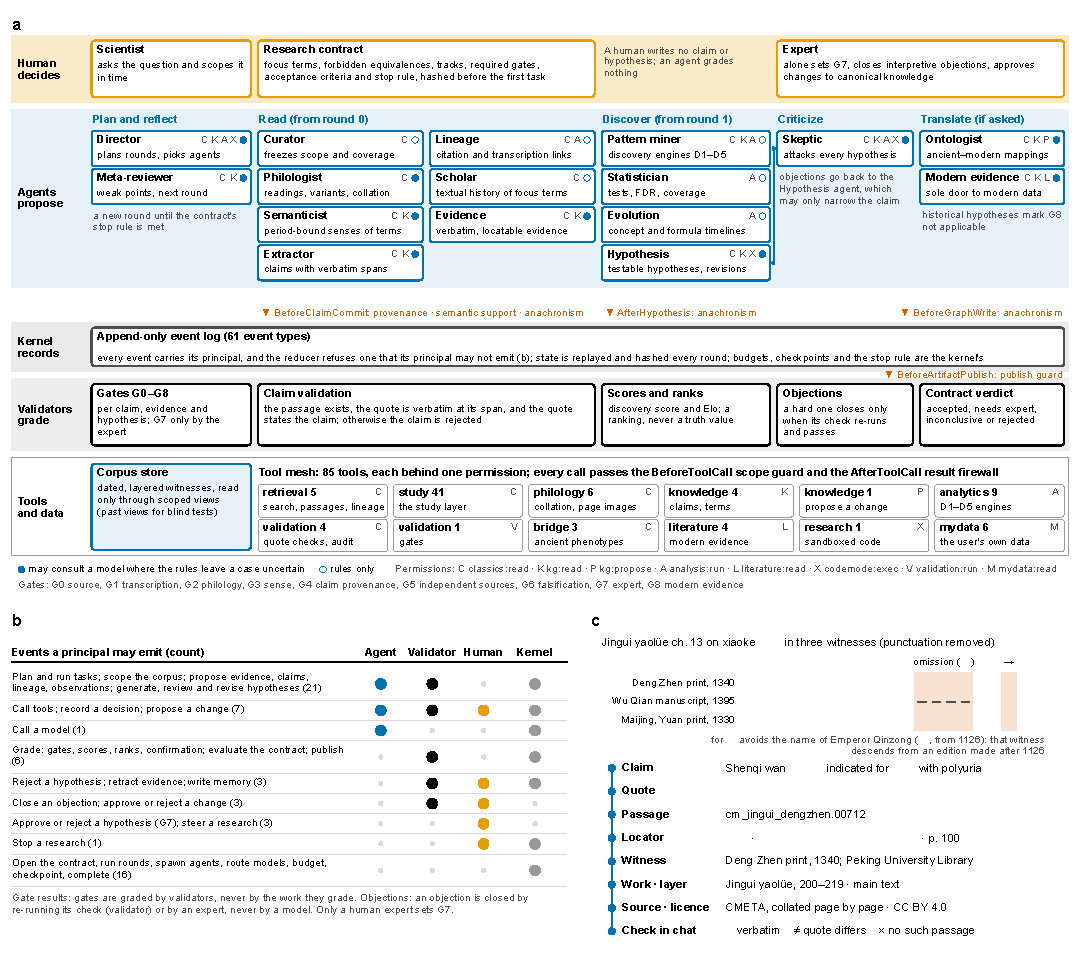
\includegraphics[width=1\textwidth,height=\textheight]{../../../figures/out/fig1_architecture.pdf}

\textbf{Fig. 1 \textbar{} TaoChronos (道乃久): agents propose,
validators grade, experts decide.} \textbf{a}, The harness as configured
(web-canon profile), by principal (rows) and by the stage of a research
round (columns). A scientist's question becomes a research contract,
hashed before the first task. The Director plans each round and picks,
from fifteen specialists, the agents the kernel spawns; each reads only
through the research's scoped view and calls only the tools its
permissions allow (letters). Filled circles, agents that may consult a
language model where their rules leave a case uncertain (Fig. 3 called
none). The Skeptic's objections return to the Hypothesis agent, which
may only narrow a claim. Every write is an event in the log. Hooks
(vermillion) refuse a tool call or result outside the research's scope,
a claim whose quote is not verbatim or contradicts it, an equation of a
historical with a modern concept, and a report on versions the contract
never judged. Validators alone grade claims, gates G0--G6 and G8, scores
and the contract's verdict, and close a hard objection only by
re-running its check; the expert alone sets G7. \textbf{b}, Event
authority: the principals allowed to emit each group of the 61 event
types (number of types); the reducer refuses any other event.
\textbf{c}, One clause of the \emph{Jingui yaolüe} (chapter 13) in three
witnesses, aligned character by character: the Deng Zhen print (1340),
the Wu Qian manuscript (1395), which lacks 小便一斗, and the Yuan print
of the \emph{Maijing} (1330), which writes 圎 for 丸, a Song taboo form
that dates its exemplar after 1126; shaded, variant positions. Below,
the provenance chain of the first witness from claim to licence; the
conversation client checks every cited passage (✓ verbatim, ≠ quotation
differs, × no such passage). CMETA, 數位中醫校書郎. Agents, tools and
permissions: Supplementary Tables 4--8.

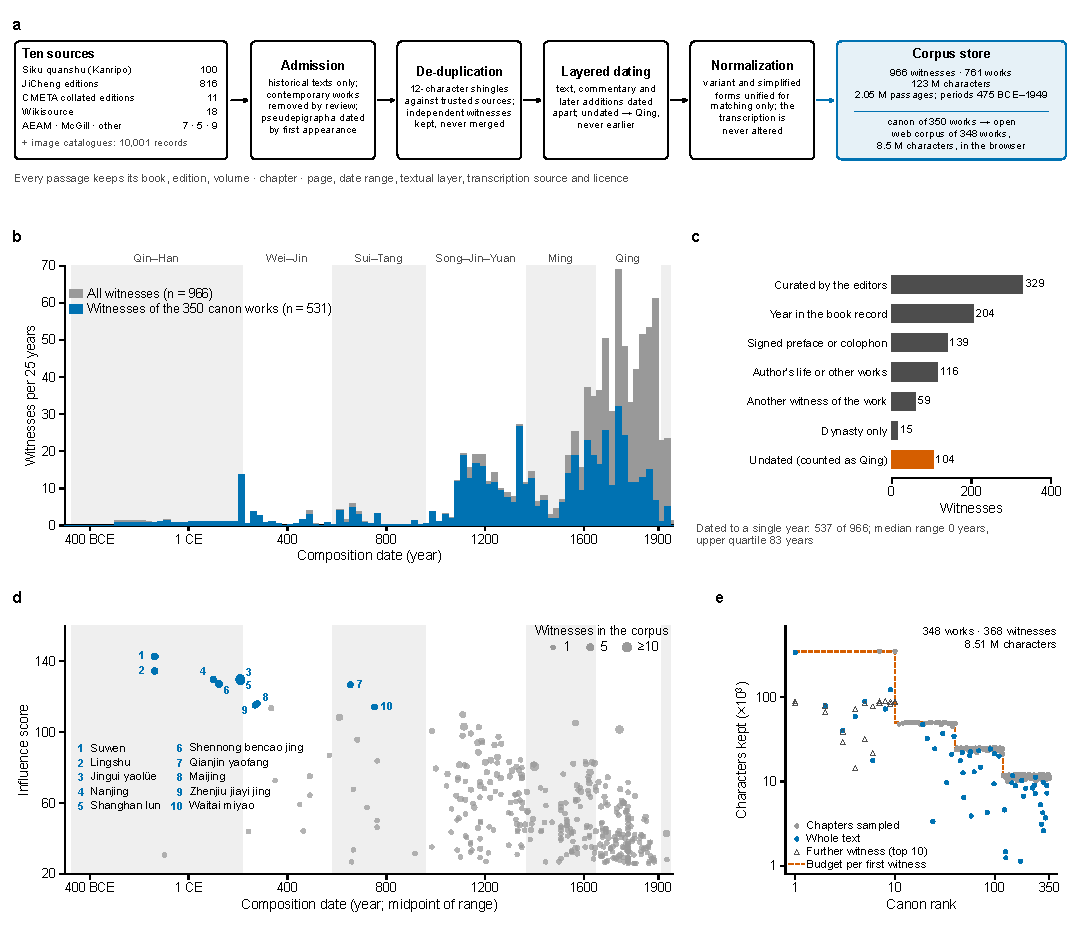
\includegraphics[width=1\textwidth,height=\textheight]{../../../figures/out/fig2_corpus.pdf}

\textbf{Fig. 2 \textbar{} A dated, layered corpus spanning two
millennia, and the canon its citations define.} \textbf{a}, Construction
of the corpus. Transcriptions from ten sources pass admission
(historical texts only), de-duplication against more trusted sources
(normalized 12-character shingles; independently collated transcriptions
are kept as separate witnesses), layer-aware dating (main text,
commentaries, editors' notes and later additions dated apart; undated
material counted as Qing, never earlier) and normalization used for
matching only. \textbf{b}, Witnesses per 25-year bin by composition
date; each witness counts once, its weight spread evenly over its date
range (n = 966; blue, the 740 witnesses of the 535 canon works). Bands
mark the analysis periods; the last, unlabelled band is the Republican
period (1912--1949). \textbf{c}, Basis on which each witness was dated;
the 104 undated witnesses are counted as Qing (vermillion), never
earlier. \textbf{d}, Influence score of the 535 canon works against the
midpoint of their composition range; point area, witnesses in the corpus
(capped at 10). Score = 10 log₂(1 + citing works not older than it) + 2
× periods in which it is cited + 2 log₂(1 + citations) + 3 log₂(1 +
witnesses) + 6 × inclusion in the \emph{Siku quanshu}; the ten highest
(blue) are keyed by rank. Later works have had fewer chances to be
cited: the score describes what the corpus cites, not a verdict on the
tradition. \textbf{e}, Characters kept for each witness of the open web
corpus against the canon rank of its work (log--log). Dashed line, the
budget of a work's first witness (350,000 characters for ranks 1--10,
then 50,000, 25,000 and 12,000); blue, texts kept whole; triangles,
second and third witnesses of the ten highest-ranked works. Data: corpus
catalogues (\texttt{corpus/catalog}) and the web corpus pack
(\texttt{corpus/web}).

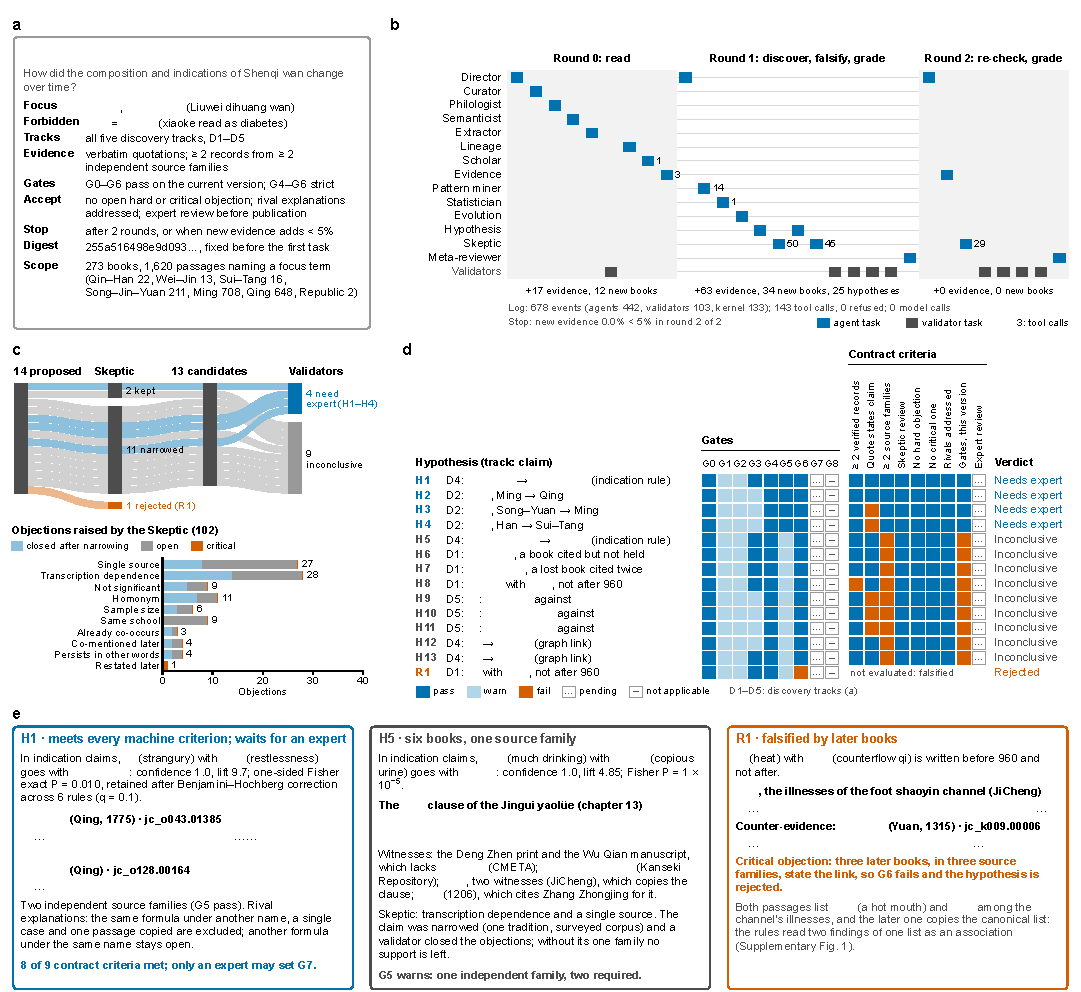
\includegraphics[width=1\textwidth,height=\textheight]{../../../figures/out/fig3_end_to_end.pdf}

\textbf{Fig. 3 \textbar{} One research question, end to end.}
\textbf{a}, The question, put to the harness on the open canon corpus
(web-canon profile; rules only, no model called), and the contract fixed
before the first task. \textbf{b}, The 30 tasks in the order the
Director planned them over three rounds: agent tasks (blue), validator
tasks (grey); numbers, tool calls. Below each round, the evidence
records, new books and hypotheses it added; the run stopped after the
last round the contract allowed, which added no evidence. \textbf{c},
The 14 hypotheses proposed in round 1: the Skeptic kept 2, sent 11 back
to be narrowed and rejected 1; validators then judged the 13 candidates.
Below, the Skeptic's 102 objections by check: closed by a validator once
the claim was narrowed, left open, or critical. \textbf{d}, The final
hypotheses against the gates and the contract's criteria. H1 and H2 meet
every criterion a machine can check; H3 and H4 rest in part on a
quotation that does not clearly state its claim, which the contract
leaves to an expert. Nine fail on independent sources (G5): passage
reuse, closed transitively, puts 36 of the 46 evidence books into one
source family (Supplementary Fig. 1). \textbf{e}, Three outcomes with
their verbatim evidence. H1 waits for an expert. H5 rests on six books
of one family: the 消渴 clause of the \emph{Jingui yaolüe}, its
witnesses and copies. R1 is rejected because three later books state the
link; they copy the canonical list of the kidney channel's illnesses
that the earlier passage holds, and the rules read two findings of one
list as an association. A second run writes the same report; report,
event log, hypotheses and objections: Supplementary Data 1--2 and
Supplementary Tables 9--10. D1--D5, discovery tracks: lost knowledge,
concept evolution, formula evolution, hidden associations,
contradictions.

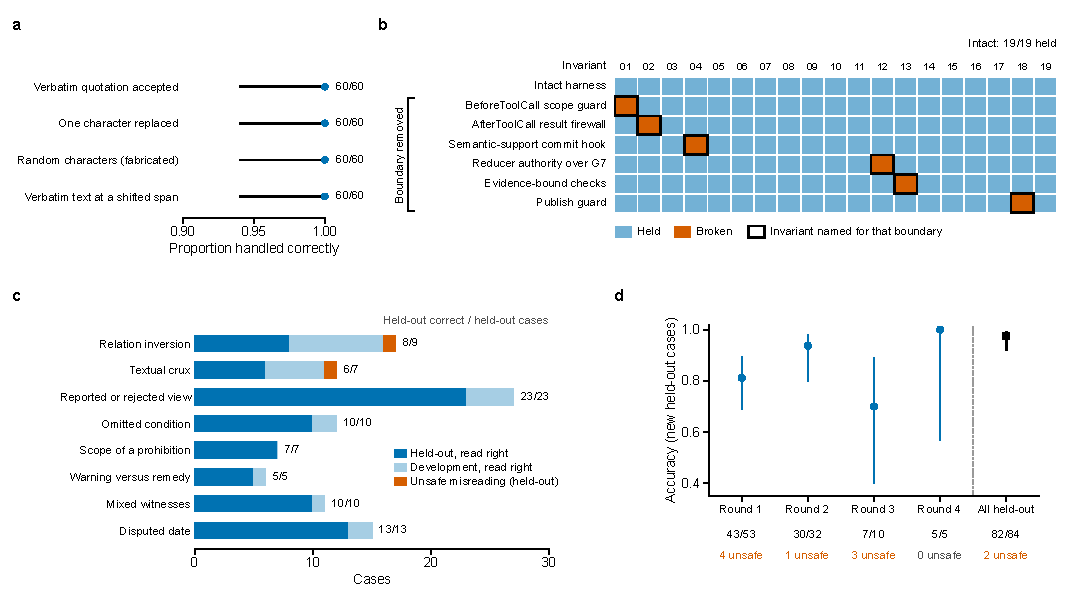
\includegraphics[width=1\textwidth,height=\textheight]{../../../figures/out/fig4_verification.pdf}

\textbf{Fig. 4 \textbar{} Quotations stay verbatim, the harness's
boundaries hold, and hard readings stay safe.} \textbf{a}, Quotation
checks on 60 random passages of the demonstration corpus: verbatim
quotations accepted; quotations with one character replaced, of random
characters, or verbatim at a shifted span rejected. Dots, proportions;
lines, Wilson 95\% confidence intervals. \textbf{b}, Nineteen invariants
(I01--I19) run as probes on the intact harness and on six variants, each
with one boundary removed by deleting its check at run time. Every
removal broke the invariant named for its boundary (outlined) and no
other; 127 of 133 cells held. In three cases a second safeguard limited
the damage: without the scope guard the tool it no longer refused
returned nothing of the withheld passage; forged G7 events reached the
log but not the state; without the bound checks two of five impossible
evidence records verified. \textbf{c}, 107 hard interpretive cases in
eight classes, each a verbatim quotation with one correct reading
(development, 23 cases used to write the rules; held-out, 84). Numbers,
held-out cases read correctly. Both errors were unsafe, a reading that
commentators dispute accepted as supported (the Dahuang mudan tang
clause and the 里水 of the Yuebi jia zhu tang clause); they are
reported, not patched. \textbf{d}, Accuracy in four blind rounds, each
on new cases written before the rules that first read them, and on all
held-out cases under the current rules. Lines, Wilson 95\% confidence
intervals; below, correct/total and unsafe errors. Data:
\texttt{taochronos\ eval} on the demonstration corpus (\textbf{a},
\textbf{c}), \texttt{paper/figures/mutation\_matrix.py} (\textbf{b}) and
\texttt{docs/evals.md} (\textbf{d}).

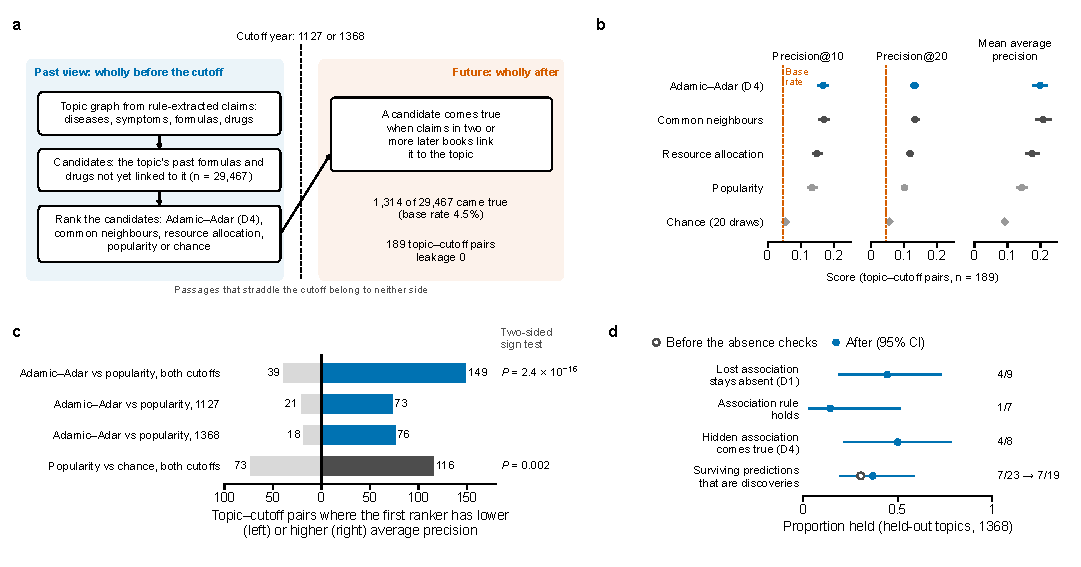
\includegraphics[width=1\textwidth,height=\textheight]{../../../figures/out/fig5_research_value.pdf}

\textbf{Fig. 5 \textbar{} Rankings computed from the past anticipate the
links later physicians wrote.} \textbf{a}, Blind temporal benchmark on
the full corpus. At each cutoff (1127, 1368) the store splits into
passages dated wholly before and wholly after it; passages that straddle
it belong to neither side. For every disease or symptom of the lexicon
with 150--6,000 past and at least 300 future passages, the formulas and
drugs of its past graph not yet linked to it are ranked; a candidate
comes true when claims in two or more later books link it to the topic.
\textbf{b}, Precision at 10 and 20 and mean average precision of five
rankers over the 189 topic--cutoff pairs in which at least one link came
true. Dots, means; lines, 95\% confidence intervals; chance, 20 random
rankings; dashed line, base rate (4.5\%). \textbf{c}, Paired comparisons
of average precision over topic--cutoff pairs; two-sided sign tests, one
tie excluded. \textbf{d}, Predictions of the whole pipeline run on the
past view at 1368 for four held-out topics (胸痹, 霍乱, 虚劳, 痰饮):
proportion borne out by later books, with Wilson 95\% confidence
intervals. Open circle, before the absence checks, which rejected two
wrong `lost' and two already attested `hidden' associations and no
discovery. No passage outside the past view was read (leakage 0). Values
of the full-corpus run documented in \texttt{docs/evals.md}; the full
store is not distributed, and Supplementary Fig. 3 repeats the benchmark
on the open corpus.

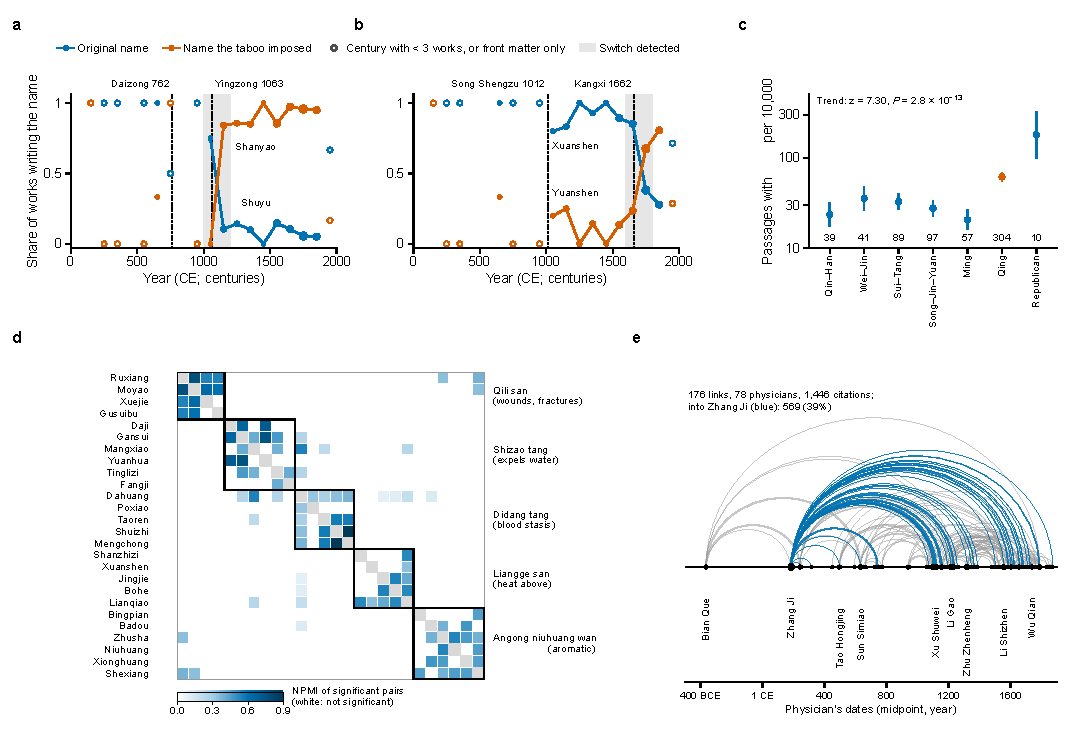
\includegraphics[width=1\textwidth,height=\textheight]{../../../figures/out/fig6_case_studies.pdf}

\textbf{Fig. 6 \textbar{} On the open canon corpus, the study layer
recovers history written into the texts.} All panels are computed by the
deterministic study layer on the open web corpus (533 works, 168,278
passages). \textbf{a}, \textbf{b}, Share of works per century writing an
original drug name and the name a naming taboo imposed: 薯蓣 and 山药
(\textbf{a}), 玄参 and 元参 (\textbf{b}). Dashed lines, the years from
which the names were avoided: Tang Daizong (李豫, 762) and Song Yingzong
(赵曙, 1063) in \textbf{a}; the Song ancestor Shengzu (赵玄朗, 1012) and
the Kangxi emperor (玄烨, 1662) in \textbf{b}; shading, the switch
interval the tool detected; marker area, works in the century; open
markers, centuries with fewer than three works or only undated front
matter dated conservatively to 1911. A work writing both names counts
for both. \textbf{c}, Passages mentioning 温病 (warm disease) per 10,000
passages by period, with Wilson 95\% confidence intervals; numbers,
passages with the term. Two-sided Cochran--Armitage test for trend
across the ordered periods. \textbf{d}, Normalized pointwise mutual
information (NPMI) of drug pairs co-occurring significantly in 4,554
compositions (a composition repeated in copies of one work counted once;
pairs in at least ten works tested; one-sided Fisher exact test,
Benjamini--Hochberg q \textless{} 0.05; 1,184 pairs). Groups are
communities of the strong pairs (NPMI ≥ 0.3), found without formula
names; shown (outlined) are the five of twelve whose drugs hold together
most tightly (mean NPMI of their significant pairs). Each holds the core
of a classical formula (right); liquorice (甘草), present in 43\% of
compositions, joins none. \textbf{e}, Citations between physicians: arcs
join citing and cited physicians placed at the midpoints of their dates;
width ∝ √citations; blue, citations of Zhang Ji (张机). Five links whose
cited physician lived after the citing one (28 citations) are omitted as
chronologically impossible.

\hypertarget{tables}{%
\section{Tables}\label{tables}}

\textbf{Table 1 \textbar{} Eight ways an agent can go wrong on the
classical literature, the mechanism that stops each in TaoChronos, and
the measured evidence that it does}

\begin{longtable}[]{@{}
  >{\raggedright\arraybackslash}p{(\columnwidth - 6\tabcolsep) * \real{0.2500}}
  >{\raggedright\arraybackslash}p{(\columnwidth - 6\tabcolsep) * \real{0.2500}}
  >{\raggedright\arraybackslash}p{(\columnwidth - 6\tabcolsep) * \real{0.2500}}
  >{\raggedright\arraybackslash}p{(\columnwidth - 6\tabcolsep) * \real{0.2500}}@{}}
\toprule\noalign{}
\begin{minipage}[b]{\linewidth}\raggedright
Failure mode
\end{minipage} & \begin{minipage}[b]{\linewidth}\raggedright
Example in the classics
\end{minipage} & \begin{minipage}[b]{\linewidth}\raggedright
Mechanism in TaoChronos
\end{minipage} & \begin{minipage}[b]{\linewidth}\raggedright
Evidence in this study
\end{minipage} \\
\midrule\noalign{}
\endhead
\bottomrule\noalign{}
\endlastfoot
Fabricated or altered quotation & A quote with one character changed, or
the right words at the wrong place & The harness, not the producer,
locates every quote in its passage at commit (verbatim, or after
length-preserving variant normalization); the conversation client checks
every cited passage & 180/180 corrupted quotations rejected, 60/60
verbatim accepted; 100\% of committed claims verbatim (Fig. 4a) \\
True quote, false reading & 「不可发汗，宜桂枝汤」 (a prohibition beside
a prescription); 「或曰\ldots 余曰非也」 (a view the author rejects) &
Semantic-support hook reads each claim's statement frame (speaker,
stance, conditions, negations) and refuses a claim its quote
contradicts; a registry of textual cruxes harvested from commentaries
makes doubtful clauses read as ambiguous & Held-out hard cases 82/84, 2
unsafe; four blind rounds (Fig. 4c,d) \\
Copies counted as independent testimony & Five witnesses of one clause
of the Jingui yaolüe and its copy in the Maijing & Gate G5 counts
independent source families (author and transcription clusters), not
books; the Skeptic checks transcription dependence and single sources &
H5 held inconclusive on one family (Fig. 3e); an over-merging of
families reported (Supplementary Fig. 1) \\
Anachronism (presentism) & Xiaoke 消渴 read as diabetes mellitus;
shanghan 伤寒 read as typhoid & Anachronism guard at claim, hypothesis
and graph-write hooks; the contract's forbidden equivalences; the
ancient--modern bridge states phenotypic similarity with typed
relations, never a retrospective diagnosis & Statements 10/10, mappings
8/8, translations 24/24; agent-asserted equivalence blocked \\
Arguments from silence & An association called lost after 960 that a
later book still states & The Skeptic searches the whole scope for
explicit, supported statements; one later statement refutes a loss and
any statement refutes a hidden link, as hard, critical objections no
rewording can close & 2 wrong lost and 2 already-written hidden
associations rejected, and no discovery (Fig. 5d); R1 rejected (Fig.
3) \\
Self-grading and premature acceptance & A model closing its own
objection, setting expert approval, or a finished run taken as an
accepted finding & Every event carries its principal and the reducer
refuses an event its principal may not emit (61 types); only validators
grade, only a human sets G7; an executable contract judges acceptance &
19/19 invariants held; each of 6 boundaries removed broke its invariant
and no other (Fig. 4b) \\
Hindsight in testing foresight & A `prediction' made after reading the
books that later confirm it & Time-machine views bounded in SQL on every
read path; passages that straddle the cutoff belong to neither side;
leakage counted, not assumed & Leakage 0; precision@10 0.168 against
0.134 (popularity) and 0.054 (chance)† (Fig. 5) \\
Irreproducible runs & A result that cannot be rerun or audited step by
step & Append-only event log replayed and hashed every round; tool-call
receipts in a hash chain; recorded model responses replayed exactly &
Resume after a crash at 4 of 4 points reaches the same state; reruns and
parallel runs identical; the end-to-end report rewritten identically \\
\end{longtable}

Every mechanism is deterministic code that runs whether a language model
or a rule produced the output; all evidence was measured with the rules
alone (no model called).

†Needs the full corpus store, which is not distributed; values from
docs/evals.md. Other values were reproduced by \texttt{taochronos\ eval}
on the demonstration corpus.

\textbf{Table 2 \textbar{} Evaluation of TaoChronos across its three
layers}

\begin{longtable}[]{@{}
  >{\raggedright\arraybackslash}p{(\columnwidth - 10\tabcolsep) * \real{0.1667}}
  >{\raggedright\arraybackslash}p{(\columnwidth - 10\tabcolsep) * \real{0.1667}}
  >{\raggedright\arraybackslash}p{(\columnwidth - 10\tabcolsep) * \real{0.1667}}
  >{\raggedright\arraybackslash}p{(\columnwidth - 10\tabcolsep) * \real{0.1667}}
  >{\raggedright\arraybackslash}p{(\columnwidth - 10\tabcolsep) * \real{0.1667}}
  >{\raggedright\arraybackslash}p{(\columnwidth - 10\tabcolsep) * \real{0.1667}}@{}}
\toprule\noalign{}
\begin{minipage}[b]{\linewidth}\raggedright
Layer
\end{minipage} & \begin{minipage}[b]{\linewidth}\raggedright
Suite
\end{minipage} & \begin{minipage}[b]{\linewidth}\raggedright
Data
\end{minipage} & \begin{minipage}[b]{\linewidth}\raggedright
Metric
\end{minipage} & \begin{minipage}[b]{\linewidth}\raggedright
Development or constructed
\end{minipage} & \begin{minipage}[b]{\linewidth}\raggedright
Held-out or real corpus
\end{minipage} \\
\midrule\noalign{}
\endhead
\bottomrule\noalign{}
\endlastfoot
Boundaries & Invariants & 19 probes of the harness under test & Held &
19/19 & Each of 6 boundaries removed breaks its invariant \\
Readings & Hard interpretive cases & 107 cases in 8 classes & Accuracy
(unsafe errors) & 23/23 (0) & 82/84 = 0.976 (2) \\
Research value† & Link anticipation & 189 topic--cutoff pairs; 29,467
candidates & Precision@10 & -- & 0.168 (popularity 0.134; chance 0.054);
higher average precision than popularity in 149 of 189, P = 2.4 ×
10⁻¹⁶ \\
& End-to-end predictions & Held-out topics, cutoff 1368 & Discoveries
among survivors & 1/8 & 7/19 = 0.37; leakage 0 \\
Verification & Fabricated quotations & 60 quotations × 4 probes &
Handled correctly & -- & 60/60 in every probe; variant spellings
accepted \\
& Provenance & Committed claims and evidence & Verbatim & -- & 100\%;
mean chain depth 7.8 levels \\
& Claim extraction & 42 gold hyperedges & Precision / recall & 1.00 /
0.976 & -- \\
& Temporal and anachronism guards & Constraints, earliest attestations,
equations & Correct & 6/6 · 6/6 · 10/10 & Leakage 0; agent-asserted
equivalence blocked \\
Deep discovery & Collation & 5 traditions copied down a known stemma &
Variant-unit recall / precision & 0.998 / 0.999 & -- \\
& Semantic reuse & 33 typed pairs & Accuracy & 0.97 & -- \\
& Stratigraphy & 5 composites; the Suwen & Layer accuracy & 0.955 &
Yunqi chapters 7/7 in the minor layer† \\
& Lost-text fragments & Constructed lost work; Qianjin yaofang &
Precision & 0.86 & 0.32† \\
Task specification & Punctuation & 55 held-out works (104 k characters)†
& Boundary F1 & -- & 0.767 (rules 0.235); characters kept 1.000 \\
& Drug pairs & 66,196 compositions† & Textbook pairs significant & -- &
7/7, lift \textgreater{} 1.5 \\
V2 & Entities (24 types) & 41 development, 25 held-out sentences & F1 &
0.991 & 0.776 \\
& Ancient phenotypes → HPO & 20 development cases; 12 random passages† &
F1 & 0.985 & 0.822 \\
& Evidence audit & 19 claims & Verdicts right (false SUPPORTED) & 19/19
(0) & -- \\
\end{longtable}

Development and constructed gold sets were written by the authors with
the rules they test; they are regression tests of intended behaviour,
not unbiased benchmarks. Only held-out and real-corpus columns estimate
generalization.

†Needs the full corpus store, which is not distributed; values from
docs/evals.md. All other values were reproduced for this paper by
\texttt{taochronos\ eval} on the demonstration corpus (40 suites, 47 s).

P value from a two-sided sign test of average precision over
topic--cutoff pairs. HPO, Human Phenotype Ontology.

\end{document}
